\documentclass[../Main.tex]{subfiles}

\graphicspath{{\subfix{../Figures_and_Tables/}}}
 
\begin{document}

\newpage
\begin{figure}[t]
	\begin{center}
	\caption{\label{fig:nh_con_map} \centering Nursing Home Certificate-of-Need Regulation in the United States}
    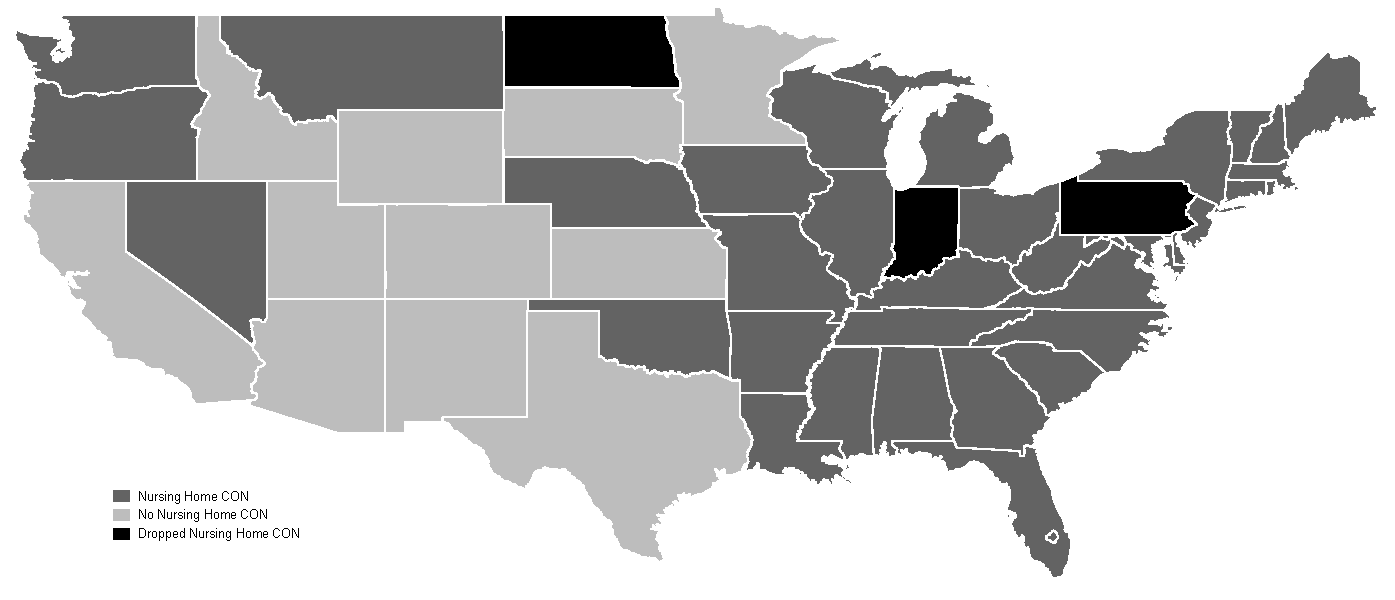
\includegraphics[width=\textwidth,keepaspectratio]{CON_Map.pdf}
    \end{center}
    \footnotesize
		\textit{Notes}: This figure shows which states dropped NH-CON regulations during our sample period (black), and which states did (dark gray) and did not (light gray) have NH-CON regulations during our sample period. All of the states that had NH-CON during our sample period except Connecticut and Louisiana, both of which adopted NH-CON during the sample period, were included in our donor pool of potential controls when finding synthetic matches for the states that dropped NH-CON. Data source: American Health Planning Association (AHPA), compiled by \citet{stratmann2014certificate}, and the National Conference of State Legislatures.
\end{figure}
\clearpage


\newpage
\begin{figure}[t]
    \begin{center}
	\caption{\label{fig:model_graph} The Effect of Nursing Home CON on Nursing Home Quality}
	\begin{tikzpicture}[scale=1]
    % Axis
    \coordinate (y) at (0,9);
    \coordinate (x) at (10,0);
    \draw[<->] (y) node[above] {$c_z'(z_i)$} -- (0,0) --  (x) node[right] {$z_i$};
    \node [above] at (0,9.6) {$MB(z_i)$,};
    % Draw help grid
    %\draw[step=10mm, lightgray] (0,0) grid (10,10); 
    % define some coordinates
    %\path
    \coordinate (cstart) at (0,0);
    \coordinate (cend) at (10,8);
    \coordinate (mb0start) at (0,2.5);
    \coordinate (mb0end) at (10,6);
    \coordinate (mb1start) at (0,1.5);
    \coordinate (mb1end) at (10,5);
    % Draw the lines
     \draw[thick, name path=c] (cstart) to[bend right = 30] (cend) node[right] {$c_z'(z_i)$};
     \draw[thick, name path=mb0] (mb0start) to[bend left = 15] (mb0end) node[right] {$MB^{No~CON}(z_i)$};
     \draw[thick, name path=mb1] (mb1start) to[bend left = 15] (mb1end) node[right] {$MB^{CON}(z_i)$};
     \path[name intersections={of=c and mb0, by=eq0}];
     \draw[black,fill] (eq0) circle[radius = 2pt];
    \draw[thick, dotted] (eq0) -- (eq0 |- 0,0) node[below,xshift=.5cm]{$z_i^{*No~CON}$};
    \path[name intersections={of=c and mb1, by=eq1}];
     \draw[black,fill] (eq1) circle[radius = 2pt];
    \draw[thick, dotted] (eq1) -- (eq1 |- 0,0) node[below,xshift=-.2cm]{$z_i^{*CON}$};
\end{tikzpicture}\\
		\end{center}
		\footnotesize
		\textit{Notes}: This figure shows graphically the effect of implementing NH-CON regulations on nursing home quality. $MB^{No~CON}(z_i)$ and $MB^{CON}(z_i)$ represent the marginal benefit of increasing quality with and without NH-CON, and are equal to $\frac{\partial [\prod_{j\neq i} prob(z_i^* -z_j > b_{ji})]}{\partial z_i}(P-c)$ and  $\frac{\partial [\prod_{j\neq i} prob(z_i^* -z_j > b_{ji})]}{\partial z_i}(P-c-R)$, respectively. $c_z'(z_i)=\frac{\partial c_z(z_i^*)}{\partial z_i}$ represents the marginal cost of increasing quality. The implementation of NH-CON leads to a reduction in the equilibrium nursing home quality. Similarly, the repeal of NH-CON leads to an increase in the equilibrium nursing home quality.
	\end{figure}
\clearpage

%%%%%%%%%%%%%%%% Q Nursing Homes %%%%%%%%%%%%%%%%%%%%%

% q_nh_plots_pa
\newpage
\begin{figure}[t] 
	\begin{center}
	\caption{\label{fig:q_nh_plots_pa} \centering A Comparison Between DID, SC, and SDID Estimates for the Effect of Dropping NH-CON Regulations on the Quantity of Nursing Homes Per 100,000 in Pennsylvania}
    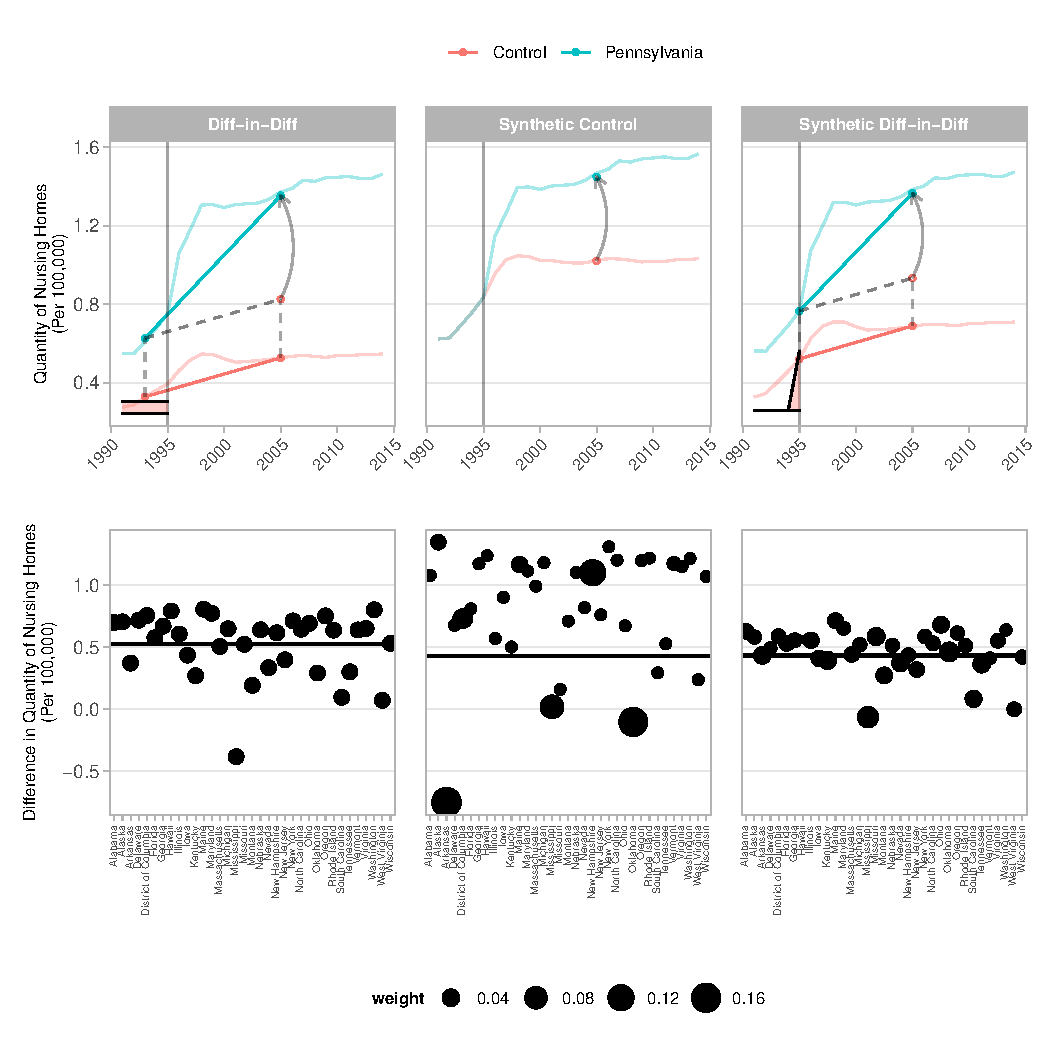
\includegraphics[width=\textwidth,keepaspectratio]{Synth_DID_Analysis/q_nursing_homes_plots_PA.pdf}
    \end{center}
    \footnotesize
		\textit{Notes}: The plots in the first row show trends in the quantity of nursing homes per 100,000 over time for Pennsylvania and the relevant weighted average of control states, with the weights used to average pre-treatment time periods at the bottom of the plots. The curved arrows in the first row indicate the estimated average treatment effect, $\hat{\tau}$ from equation (\ref{eq:ave_effect_deltas}), and the vertical lines represent the year prior to PA dropping NH-CON regulations. The plots in the second row show the state-by-state adjusted outcome difference $\hat{\delta}_{tr}-\hat{\delta}_i$ as specified in equations (\ref{eq:sc_deltas}), (\ref{eq:did_deltas}), and (\ref{eq:sdid_deltas}), with weights $\hat{\omega}_i$ indicated by dot size, and the weighted average of these differences - the estimated effect $\hat{\tau}$ from equation (\ref{eq:ave_effect_deltas}) - indicated by the horizontal lines. Control states that get zero weight, if any, are denoted by an $\times$ symbol. Data source: 1991-2014 Centers for Medicare and Medicaid Services’ (CMS) Provider of Services files.
\end{figure}
\clearpage

% q_nh_spag_plots_pa
\newpage
\begin{figure}[t]
	\begin{center}
	\caption{\label{fig: q_nh_spag_plots_pa} \centering Placebo Analysis for the Effect of Dropping NH-CON Regulations on the Quantity of Nursing Homes Per 100,000 in Pennsylvania}
    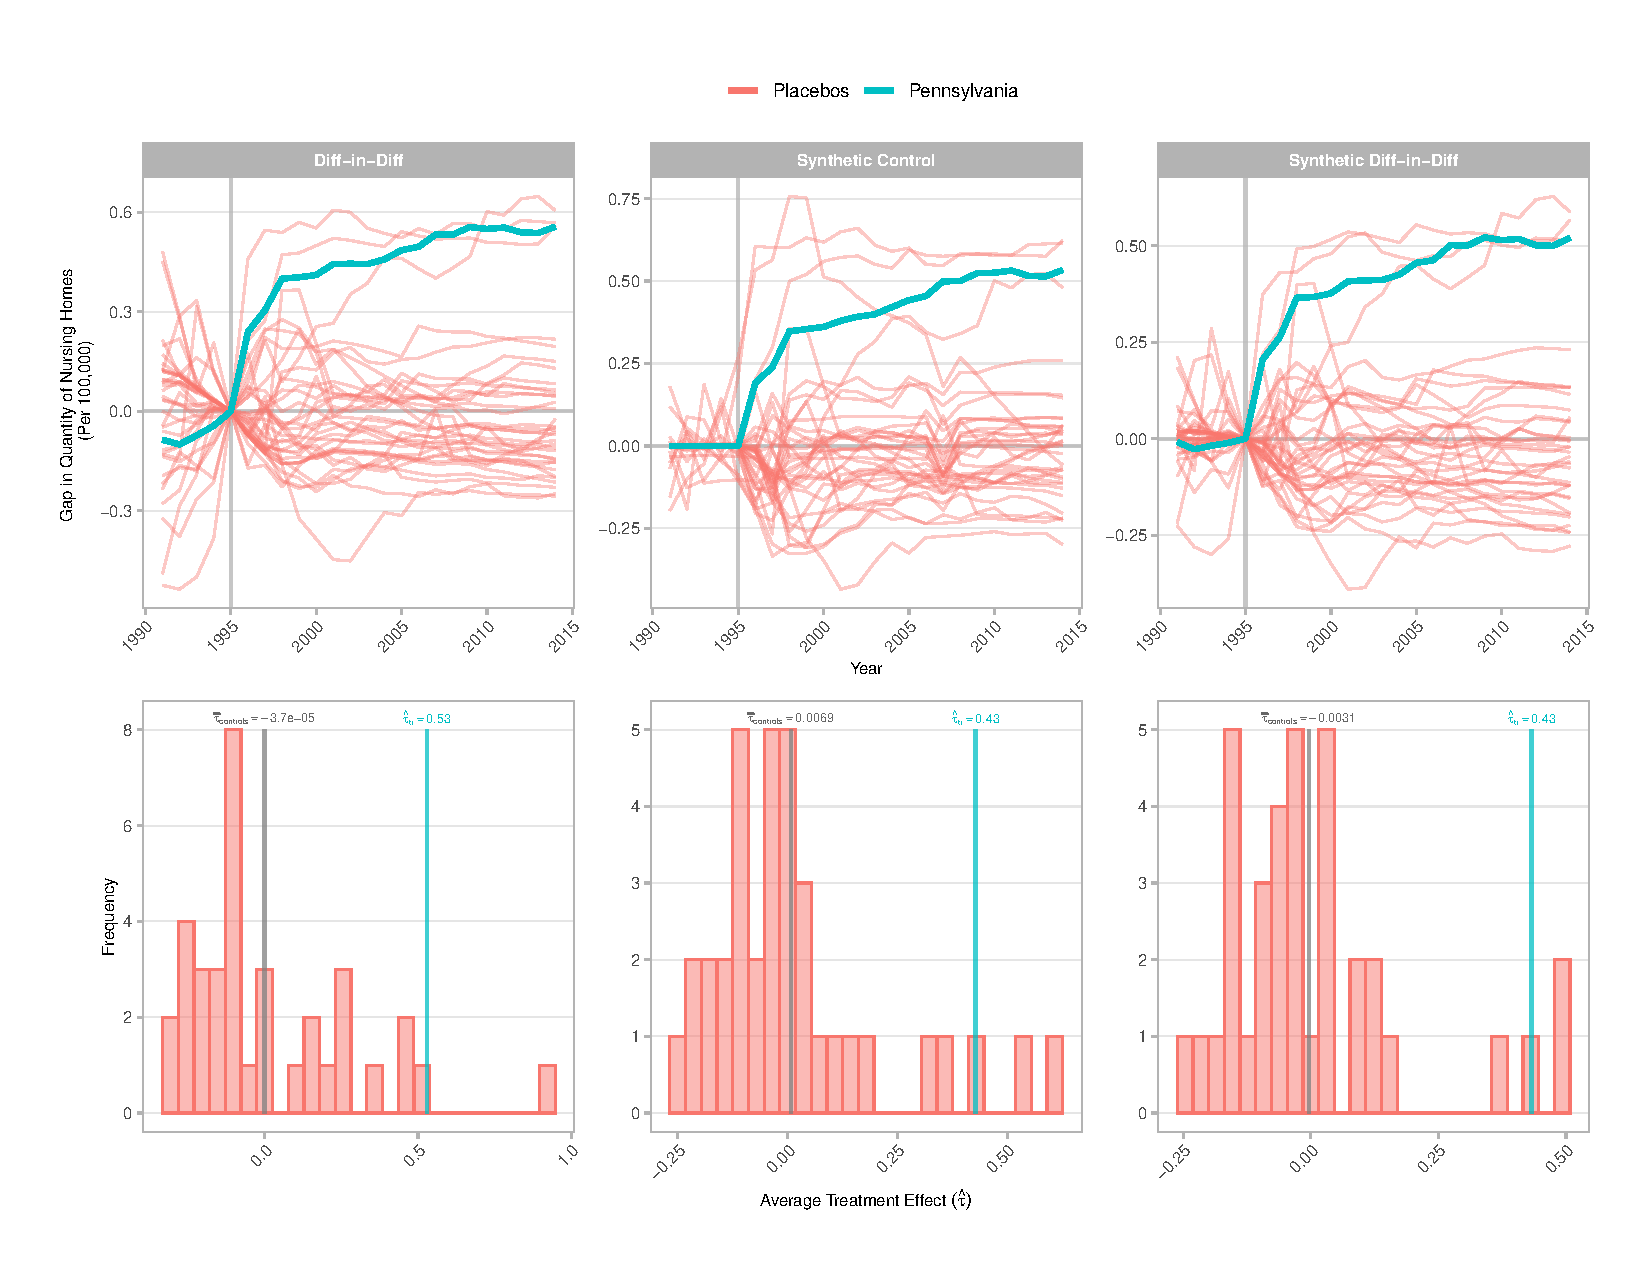
\includegraphics[width=\textwidth,keepaspectratio]{Synth_DID_Analysis/q_nh_spag_dist_plots_PA.pdf}
    \end{center}
    \footnotesize
		\textit{Notes}: The plots in the first row show the year-specific difference in the quantity of nursing homes per 100,000 between the ``treated'' state and its corresponding weighted average of control states. The thick blue line shows these gaps for PA, and the thin pink lines show these gaps for each of the placebo control states used in the placebo variance estimation procedure outlined in Algorithm \ref{alg:two}. To facilitate a better visual assessment of parallel trends, as well as a more meaningful comparison in how these gaps evolve over time, we make the gaps in the Diff-in-Diff and Synthetic Diff-in-Diff plots relative to their value in the year prior to PA dropping NH-CON regulations (as indicated by the vertical lines). We do not do this for the Synthetic Control plot because the SC weights are chosen to match the treated state's actual levels (as opposed to making the trends just parallel). Not normalizing the gaps for the Synthetic Control plot allows for a better assessment of the pre-treatment match between the treated state (or placebo ``treated'' state) and its respective synthetic control. The plots in the second row show the distribution of placebo estimates ($\hat{\tau}^{(b)}$ from Algorithm \ref{alg:two}), with the mean of the placebo estimates and the actual estimated effect for PA indicated by the gray and blue vertical lines, respectively. Data source: 1991-2014 Centers for Medicare and Medicaid Services’ (CMS) Provider of Services files.
\end{figure}
\clearpage

% q_nh_plots_in
\newpage
\begin{figure}[t] 
	\begin{center}
	\caption{\label{fig:q_nh_plots_in} \centering A Comparison Between DID, SC, and SDID Estimates for the Effect of Dropping NH-CON Regulations on the Quantity of Nursing Homes Per 100,000 in Indiana}
    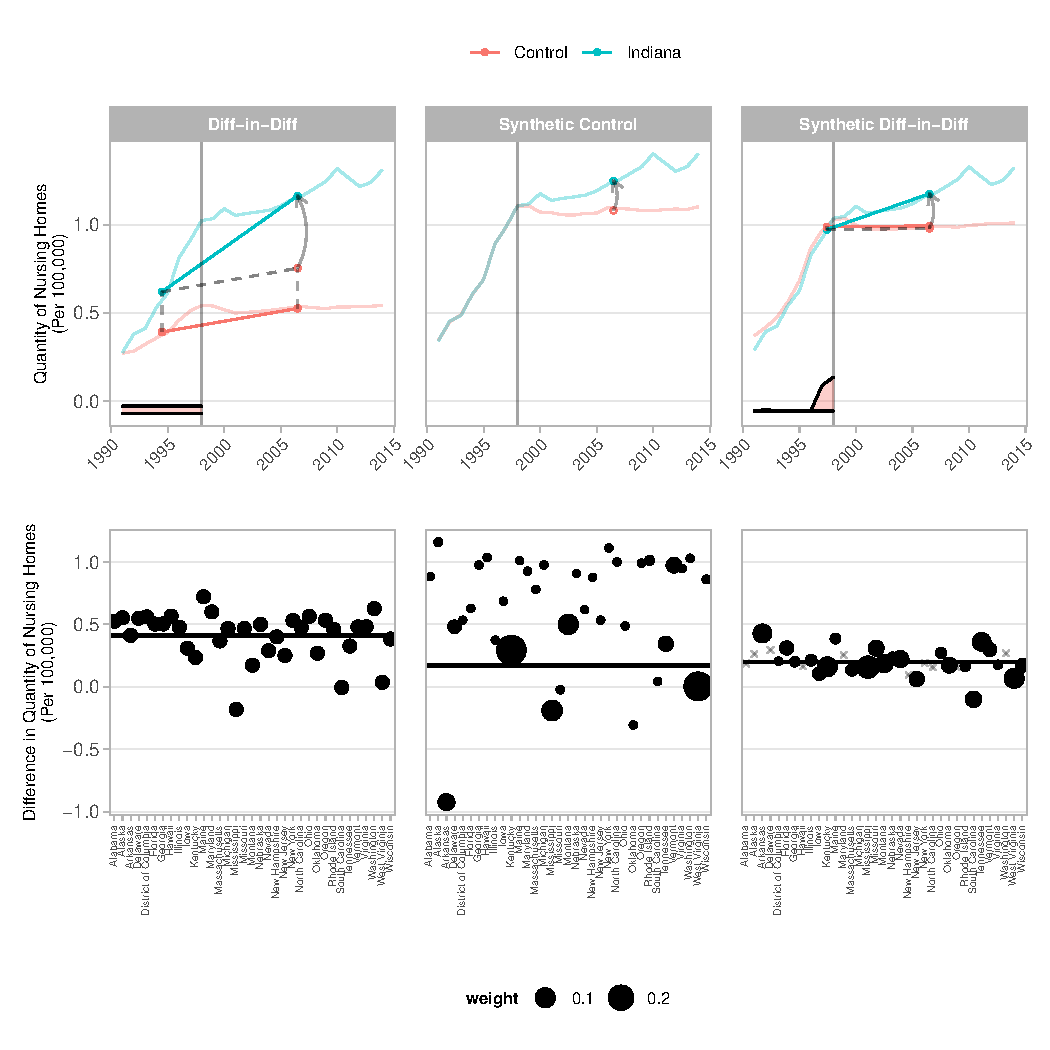
\includegraphics[width=\textwidth,keepaspectratio]{Synth_DID_Analysis/q_nursing_homes_plots_IN.pdf}
    \end{center}
    \footnotesize
		\textit{Notes}: The plots in the first row show trends in the quantity of nursing homes per 100,000 over time for Indiana and the relevant weighted average of control states, with the weights used to average pre-treatment time periods at the bottom of the plots. The curved arrows in the first row indicate the estimated average treatment effect, $\hat{\tau}$ from equation (\ref{eq:ave_effect_deltas}), and the vertical lines represent the year prior to IN dropping NH-CON regulations. The plots in the second row show the state-by-state adjusted outcome difference $\hat{\delta}_{tr}-\hat{\delta}_i$ as specified in equations (\ref{eq:sc_deltas}), (\ref{eq:did_deltas}), and (\ref{eq:sdid_deltas}), with weights $\hat{\omega}_i$ indicated by dot size, and the weighted average of these differences - the estimated effect $\hat{\tau}$ from equation (\ref{eq:ave_effect_deltas}) - indicated by the horizontal lines. Control states that get zero weight, if any, are denoted by an $\times$ symbol. Data source: 1991-2014 Centers for Medicare and Medicaid Services’ (CMS) Provider of Services files.
\end{figure}
\clearpage

% q_nh_spag_plots_in
\newpage
\begin{figure}[t]
	\begin{center}
	\caption{\label{fig: q_nh_spag_plots_in} \centering Placebo Analysis for the Effect of Dropping NH-CON Regulations on the Quantity of Nursing Homes Per 100,000 in Indiana}
    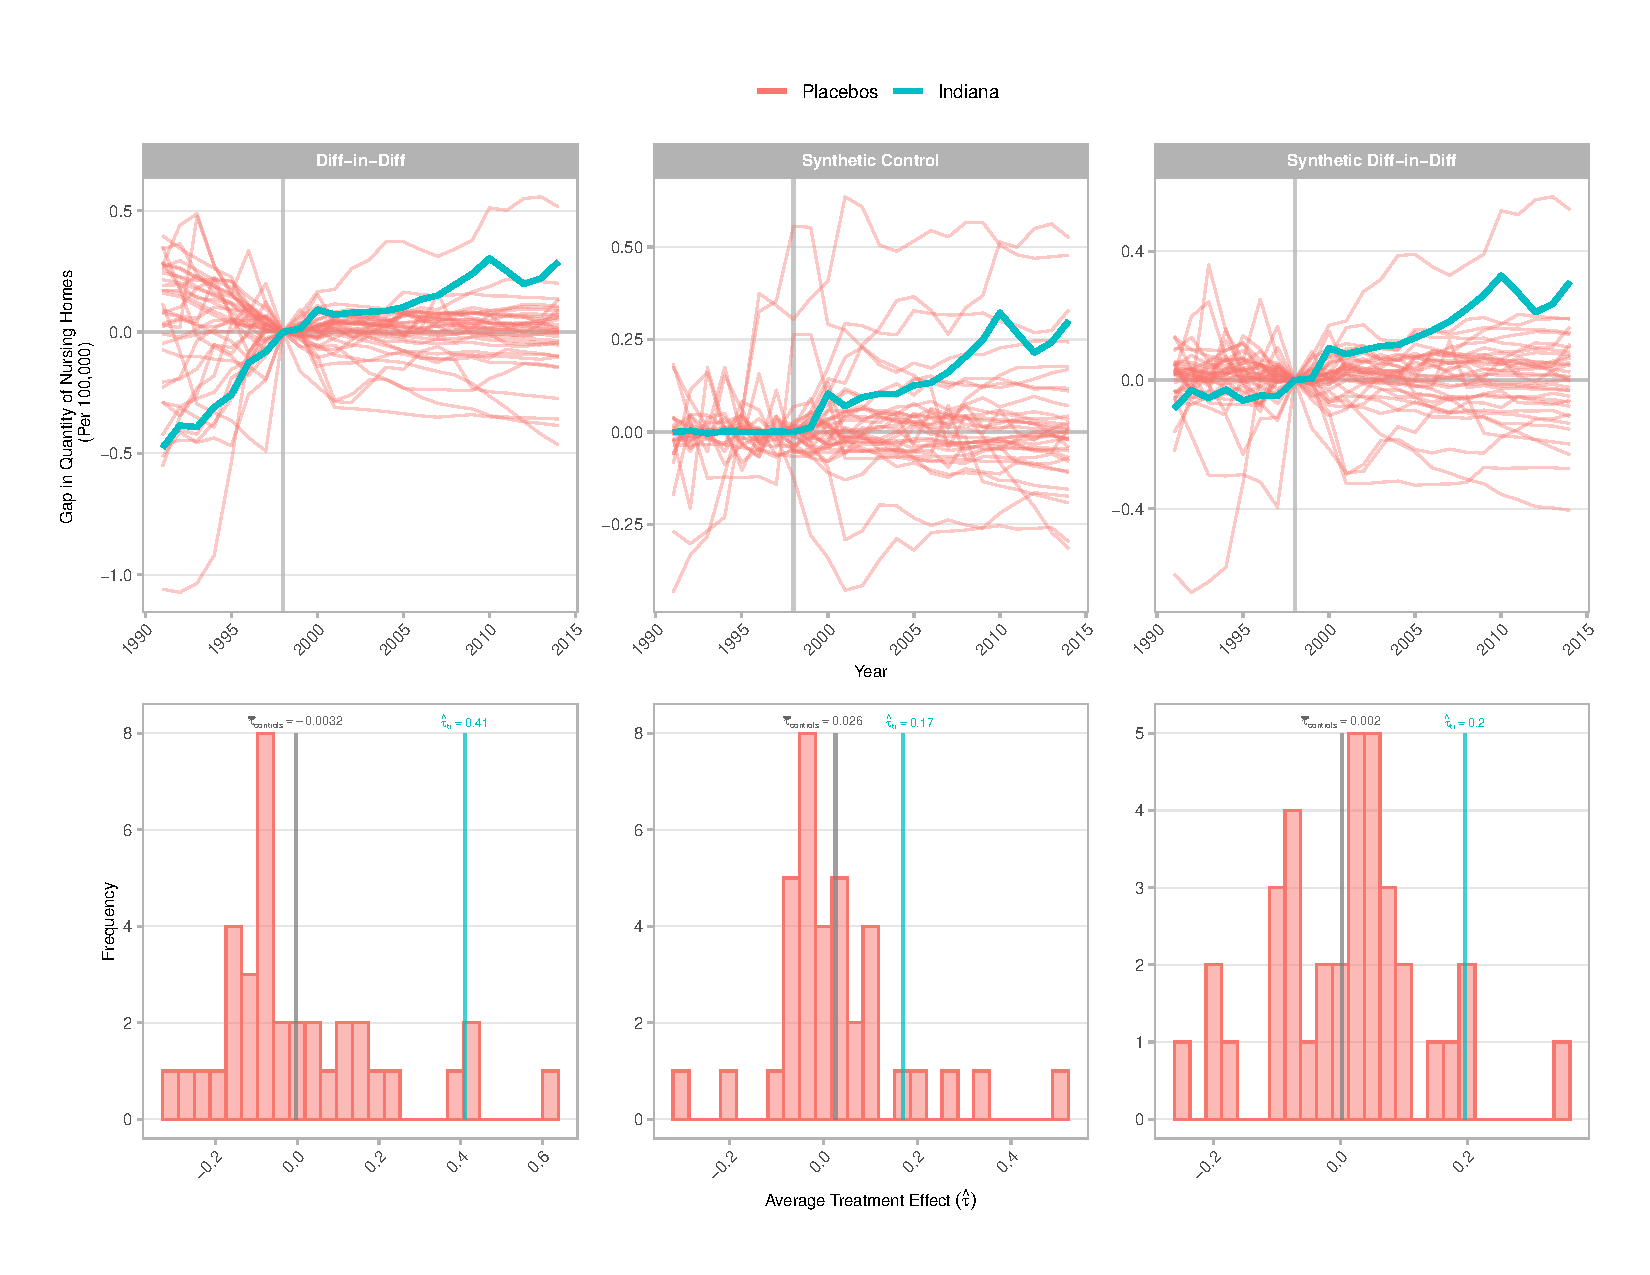
\includegraphics[width=\textwidth,keepaspectratio]{Synth_DID_Analysis/q_nh_spag_dist_plots_IN.pdf}
    \end{center}
    \footnotesize
		\textit{Notes}: The plots in the first row show the year-specific difference in the quantity of nursing homes per 100,000 between the ``treated'' state and its corresponding weighted average of control states. The thick blue line shows these gaps for IN, and the thin pink lines show these gaps for each of the placebo control states used in the placebo variance estimation procedure outlined in Algorithm \ref{alg:two}. To facilitate a better visual assessment of parallel trends, as well as a more meaningful comparison in how these gaps evolve over time, we make the gaps in the Diff-in-Diff and Synthetic Diff-in-Diff plots relative to their value in the year prior to IN dropping NH-CON regulations (as indicated by the vertical lines). We do not do this for the Synthetic Control plot because the SC weights are chosen to match the treated state's actual levels (as opposed to making the trends just parallel). Not normalizing the gaps for the Synthetic Control plot allows for a better assessment of the pre-treatment match between the treated state (or placebo ``treated'' state) and its respective synthetic control. The plots in the second row show the distribution of placebo estimates ($\hat{\tau}^{(b)}$ from Algorithm \ref{alg:two}), with the mean of the placebo estimates and the actual estimated effect for IN indicated by the gray and blue vertical lines, respectively. Data source: 1991-2014 Centers for Medicare and Medicaid Services’ (CMS) Provider of Services files.
\end{figure}
\clearpage

% q_nh_plots_nd
\newpage
\begin{figure}[t] 
	\begin{center}
	\caption{\label{fig:q_nh_plots_nd} \centering A Comparison Between DID, SC, and SDID Estimates for the Effect of Dropping NH-CON Regulations on the Quantity of Nursing Homes Per 100,000 in North Dakota}
    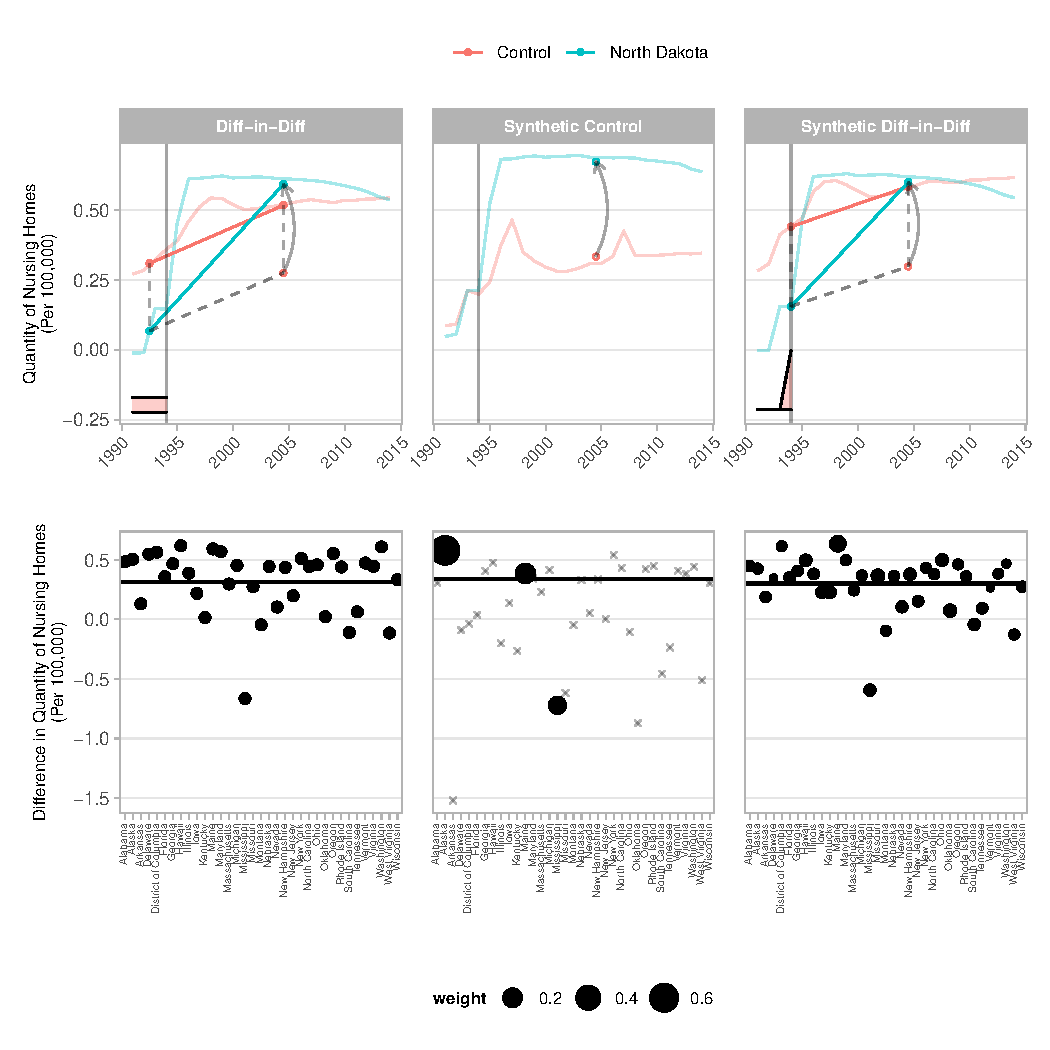
\includegraphics[width=\textwidth,keepaspectratio]{Synth_DID_Analysis/q_nursing_homes_plots_ND.pdf}
    \end{center}
    \footnotesize
		\textit{Notes}: The plots in the first row show trends in the quantity of nursing homes per 100,000 over time for North Dakota and the relevant weighted average of control states, with the weights used to average pre-treatment time periods at the bottom of the plots. The curved arrows in the first row indicate the estimated average treatment effect, $\hat{\tau}$ from equation (\ref{eq:ave_effect_deltas}), and the vertical lines represent the year prior to ND dropping NH-CON regulations. The plots in the second row show the state-by-state adjusted outcome difference $\hat{\delta}_{tr}-\hat{\delta}_i$ as specified in equations (\ref{eq:sc_deltas}), (\ref{eq:did_deltas}), and (\ref{eq:sdid_deltas}), with weights $\hat{\omega}_i$ indicated by dot size, and the weighted average of these differences - the estimated effect $\hat{\tau}$ from equation (\ref{eq:ave_effect_deltas}) - indicated by the horizontal lines. Control states that get zero weight, if any, are denoted by an $\times$ symbol. Data source: 1991-2014 Centers for Medicare and Medicaid Services’ (CMS) Provider of Services files.
\end{figure}
\clearpage

% q_nh_spag_plots_nd
\newpage
\begin{figure}[t]
	\begin{center}
	\caption{\label{fig: q_nh_spag_plots_nd} \centering Placebo Analysis for the Effect of Dropping NH-CON Regulations on the Quantity of Nursing Homes Per 100,000 in North Dakota}
    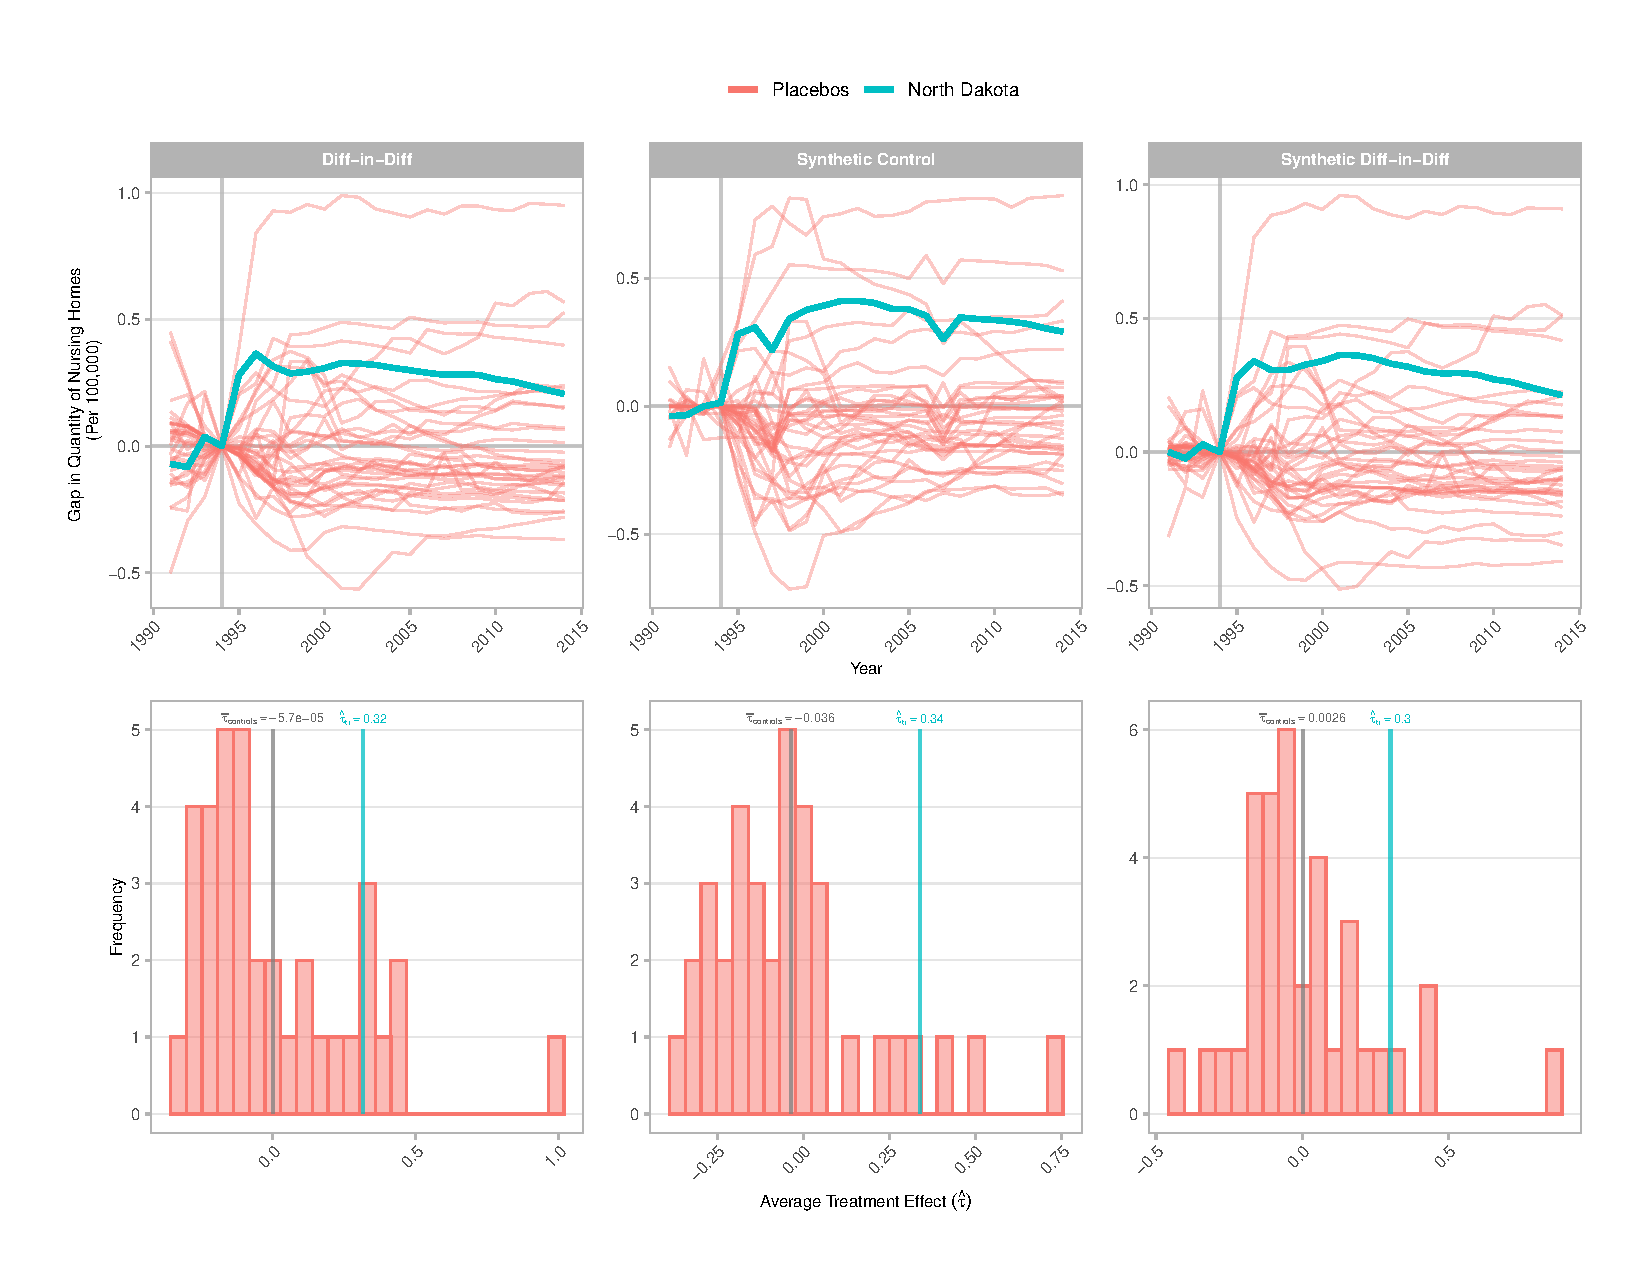
\includegraphics[width=\textwidth,keepaspectratio]{Synth_DID_Analysis/q_nh_spag_dist_plots_ND.pdf}
    \end{center}
    \footnotesize
		\textit{Notes}: The plots in the first row show the year-specific difference in the quantity of nursing homes per 100,000 between the ``treated'' state and its corresponding weighted average of control states. The thick blue line shows these gaps for ND, and the thin pink lines show these gaps for each of the placebo control states used in the placebo variance estimation procedure outlined in Algorithm \ref{alg:two}. To facilitate a better visual assessment of parallel trends, as well as a more meaningful comparison in how these gaps evolve over time, we make the gaps in the Diff-in-Diff and Synthetic Diff-in-Diff plots relative to their value in the year prior to ND dropping NH-CON regulations (as indicated by the vertical lines). We do not do this for the Synthetic Control plot because the SC weights are chosen to match the treated state's actual levels (as opposed to making the trends just parallel). Not normalizing the gaps for the Synthetic Control plot allows for a better assessment of the pre-treatment match between the treated state (or placebo ``treated'' state) and its respective synthetic control. The plots in the second row show the distribution of placebo estimates ($\hat{\tau}^{(b)}$ from Algorithm \ref{alg:two}), with the mean of the placebo estimates and the actual estimated effect for ND indicated by the gray and blue vertical lines, respectively. Data source: 1991-2014 Centers for Medicare and Medicaid Services’ (CMS) Provider of Services files.
\end{figure}
\clearpage


%%%%%%%%%%%%%%%%%%% Q Nursing Home Beds %%%%%%%%%%%%%%%%%%%

% q_nhb_plots_pa
\newpage
\begin{figure}[t] 
	\begin{center}
	\caption{\label{fig:q_nhb_plots_pa} \centering A Comparison Between DID, SC, and SDID Estimates for the Effect of Dropping NH-CON Regulations on the Quantity of Nursing Home Beds Per 100,000 in Pennsylvania}
    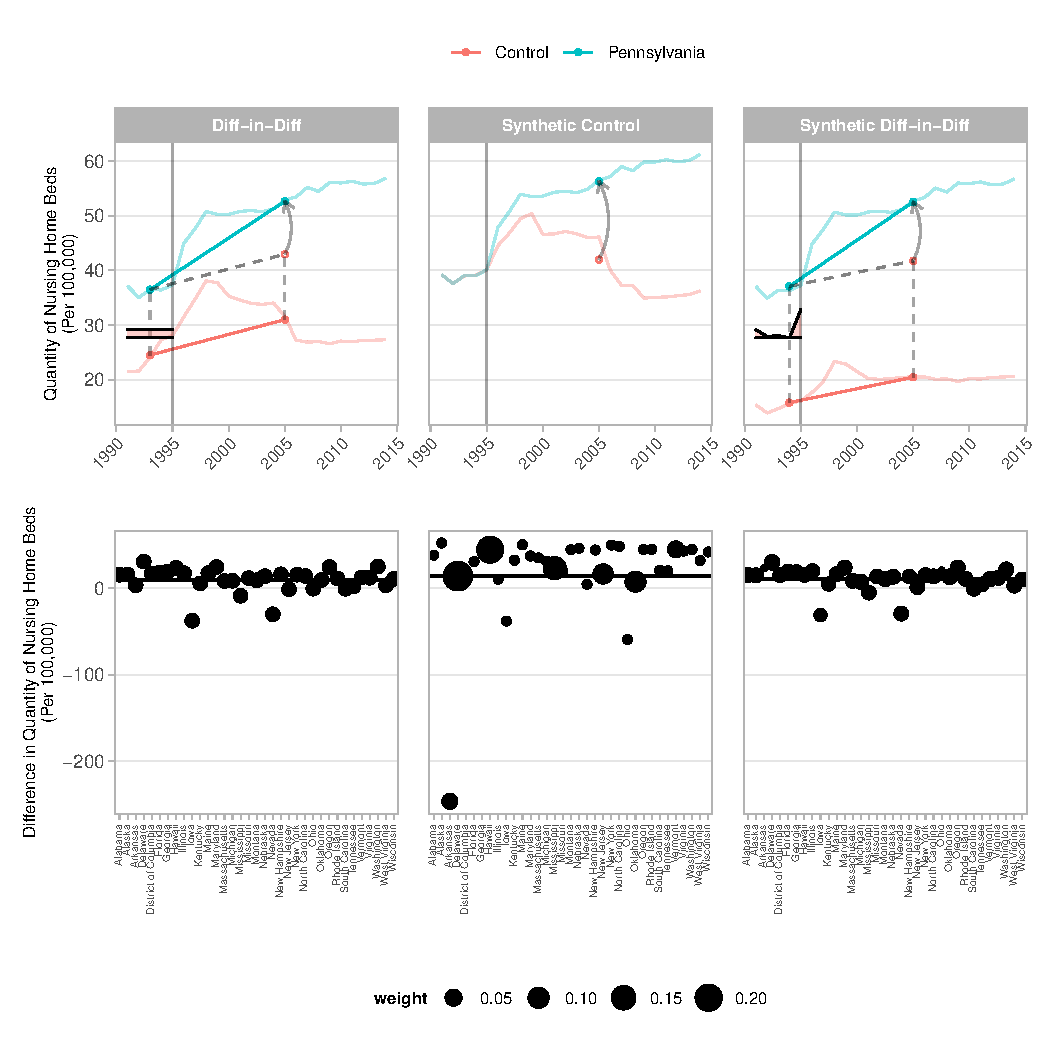
\includegraphics[width=\textwidth,keepaspectratio]{Synth_DID_Analysis/q_nursing_home_beds_plots_PA.pdf}
    \end{center}
    \footnotesize
		\textit{Notes}: The plots in the first row show trends in the quantity of nursing home beds per 100,000 over time for Pennsylvania and the relevant weighted average of control states, with the weights used to average pre-treatment time periods at the bottom of the plots. The curved arrows in the first row indicate the estimated average treatment effect, $\hat{\tau}$ from equation (\ref{eq:ave_effect_deltas}), and the vertical lines represent the year prior to PA dropping NH-CON regulations. The plots in the second row show the state-by-state adjusted outcome difference $\hat{\delta}_{tr}-\hat{\delta}_i$ as specified in equations (\ref{eq:sc_deltas}), (\ref{eq:did_deltas}), and (\ref{eq:sdid_deltas}), with weights $\hat{\omega}_i$ indicated by dot size, and the weighted average of these differences - the estimated effect $\hat{\tau}$ from equation (\ref{eq:ave_effect_deltas}) - indicated by the horizontal lines. Control states that get zero weight, if any, are denoted by an $\times$ symbol. Data source: 1991-2014 Centers for Medicare and Medicaid Services’ (CMS) Provider of Services files.
\end{figure}
\clearpage

% q_nhb_spag_plots_pa
\newpage
\begin{figure}[t]
	\begin{center}
	\caption{\label{fig: q_nhb_spag_plots_pa} \centering Placebo Analysis for the Effect of Dropping NH-CON Regulations on the Quantity of Nursing Home Beds Per 100,000 in Pennsylvania}
    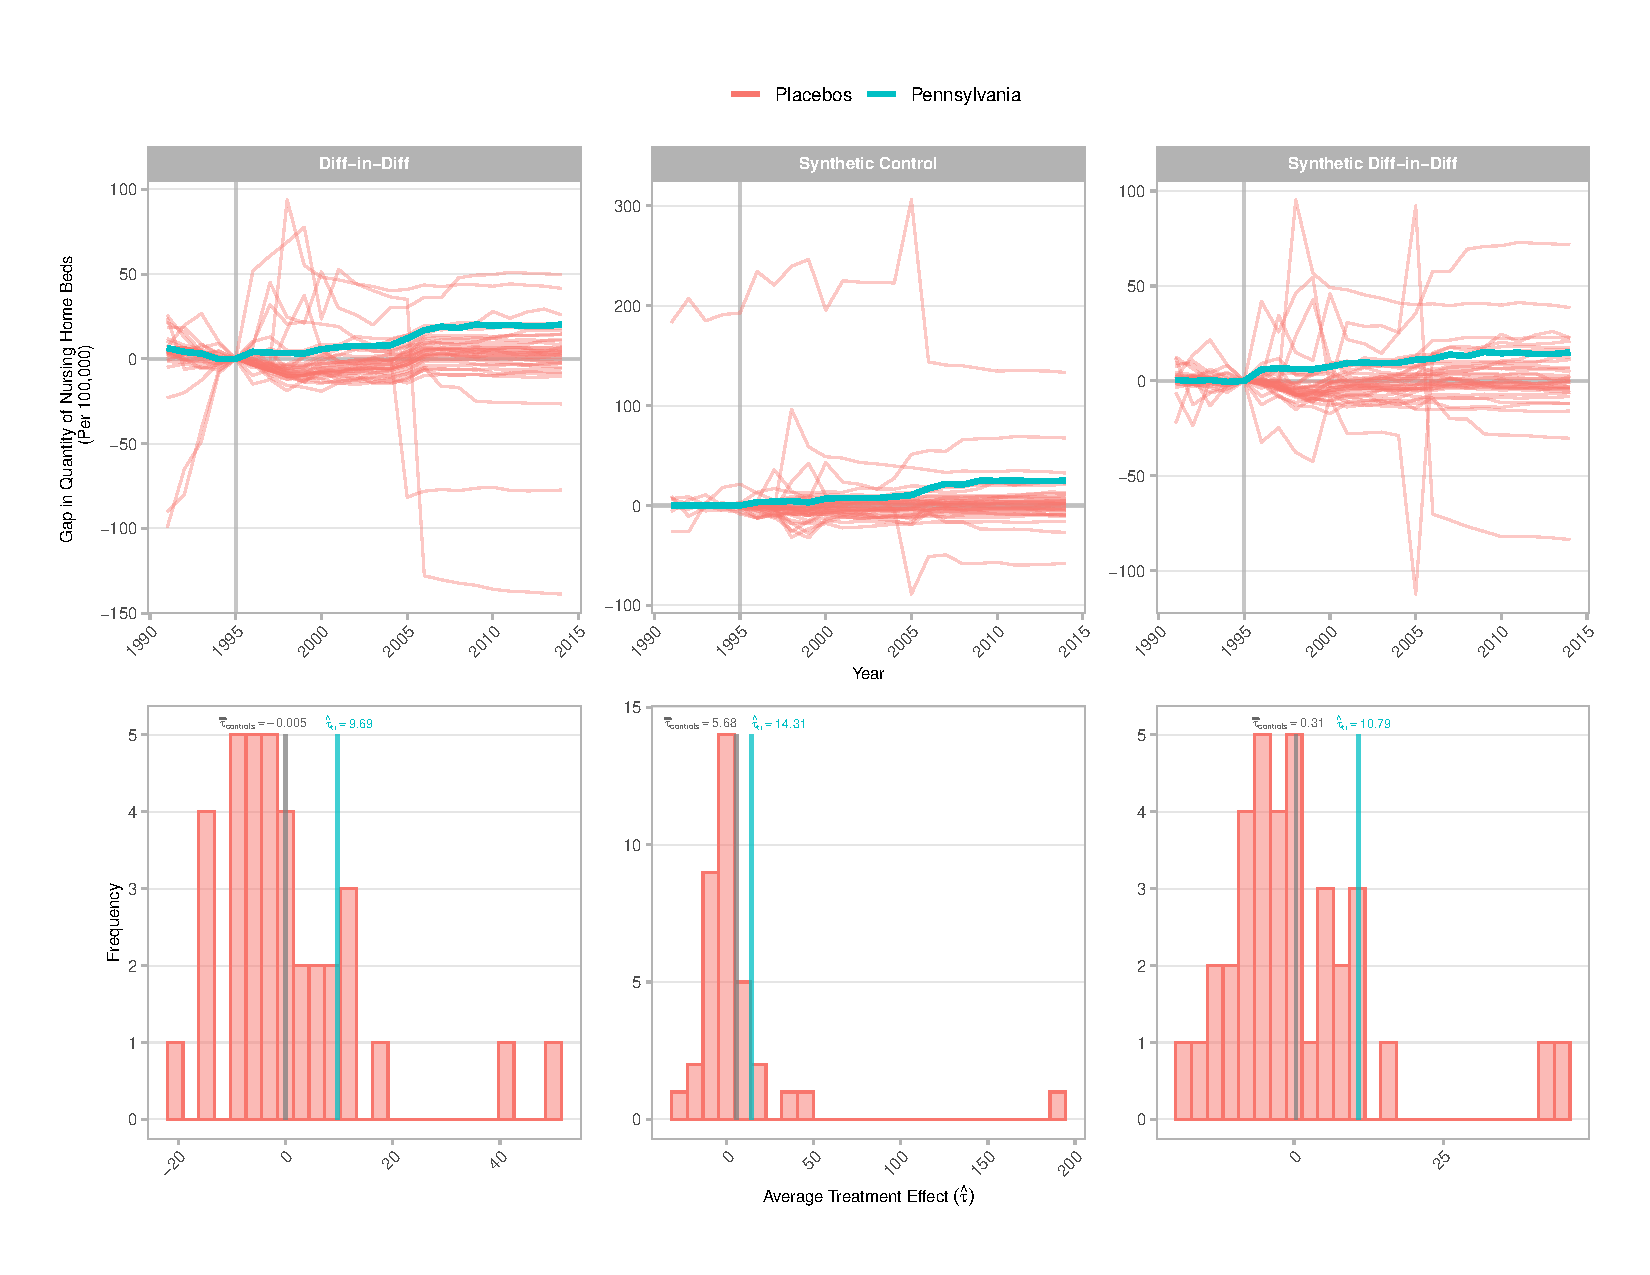
\includegraphics[width=\textwidth,keepaspectratio]{Synth_DID_Analysis/q_nhb_spag_dist_plots_PA.pdf}
    \end{center}
    \footnotesize
		\textit{Notes}: The plots in the first row show the year-specific difference in the quantity of nursing home beds per 100,000 between the ``treated'' state and its corresponding weighted average of control states. The thick blue line shows these gaps for PA, and the thin pink lines show these gaps for each of the placebo control states used in the placebo variance estimation procedure outlined in Algorithm \ref{alg:two}. To facilitate a better visual assessment of parallel trends, as well as a more meaningful comparison in how these gaps evolve over time, we make the gaps in the Diff-in-Diff and Synthetic Diff-in-Diff plots relative to their value in the year prior to PA dropping NH-CON regulations (as indicated by the vertical lines). We do not do this for the Synthetic Control plot because the SC weights are chosen to match the treated state's actual levels (as opposed to making the trends just parallel). Not normalizing the gaps for the Synthetic Control plot allows for a better assessment of the pre-treatment match between the treated state (or placebo ``treated'' state) and its respective synthetic control. The plots in the second row show the distribution of placebo estimates ($\hat{\tau}^{(b)}$ from Algorithm \ref{alg:two}), with the mean of the placebo estimates and the actual estimated effect for PA indicated by the gray and blue vertical lines, respectively. Data source: 1991-2014 Centers for Medicare and Medicaid Services’ (CMS) Provider of Services files.
\end{figure}
\clearpage

% q_nhb_plots_in
\newpage
\begin{figure}[t] 
	\begin{center}
	\caption{\label{fig:q_nhb_plots_in} \centering A Comparison Between DID, SC, and SDID Estimates for the Effect of Dropping NH-CON Regulations on the Quantity of Nursing Home Beds Per 100,000 in Indiana}
    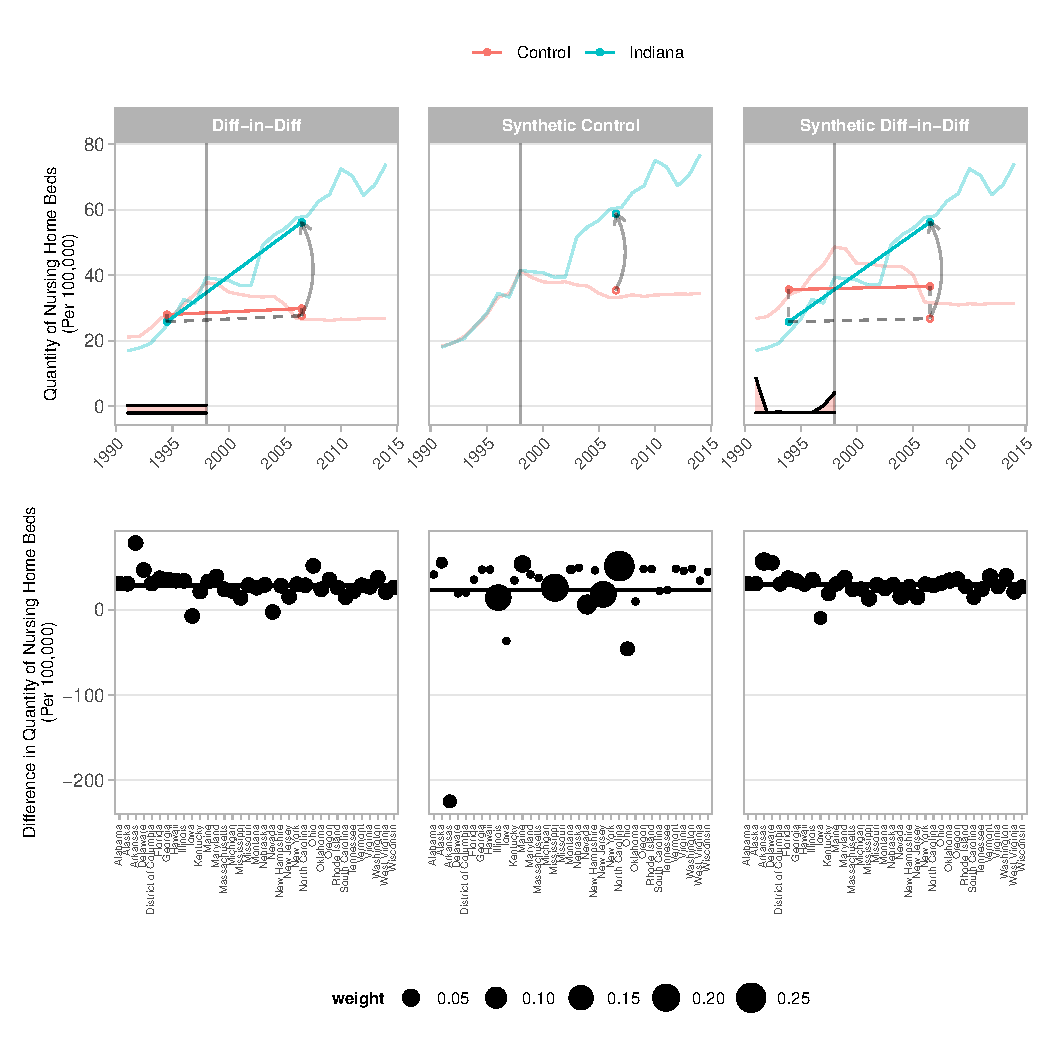
\includegraphics[width=\textwidth,keepaspectratio]{Synth_DID_Analysis/q_nursing_home_beds_plots_IN.pdf}
    \end{center}
    \footnotesize
		\textit{Notes}: The plots in the first row show trends in the quantity of nursing home beds per 100,000 over time for Indiana and the relevant weighted average of control states, with the weights used to average pre-treatment time periods at the bottom of the plots. The curved arrows in the first row indicate the estimated average treatment effect, $\hat{\tau}$ from equation (\ref{eq:ave_effect_deltas}), and the vertical lines represent the year prior to IN dropping NH-CON regulations. The plots in the second row show the state-by-state adjusted outcome difference $\hat{\delta}_{tr}-\hat{\delta}_i$ as specified in equations (\ref{eq:sc_deltas}), (\ref{eq:did_deltas}), and (\ref{eq:sdid_deltas}), with weights $\hat{\omega}_i$ indicated by dot size, and the weighted average of these differences - the estimated effect $\hat{\tau}$ from equation (\ref{eq:ave_effect_deltas}) - indicated by the horizontal lines. Control states that get zero weight, if any, are denoted by an $\times$ symbol. Data source: 1991-2014 Centers for Medicare and Medicaid Services’ (CMS) Provider of Services files.
\end{figure}
\clearpage

% q_nhb_spag_plots_in
\newpage
\begin{figure}[t]
	\begin{center}
	\caption{\label{fig: q_nhb_spag_plots_in} \centering Placebo Analysis for the Effect of Dropping NH-CON Regulations on the Quantity of Nursing Home Beds Per 100,000 in Indiana}
    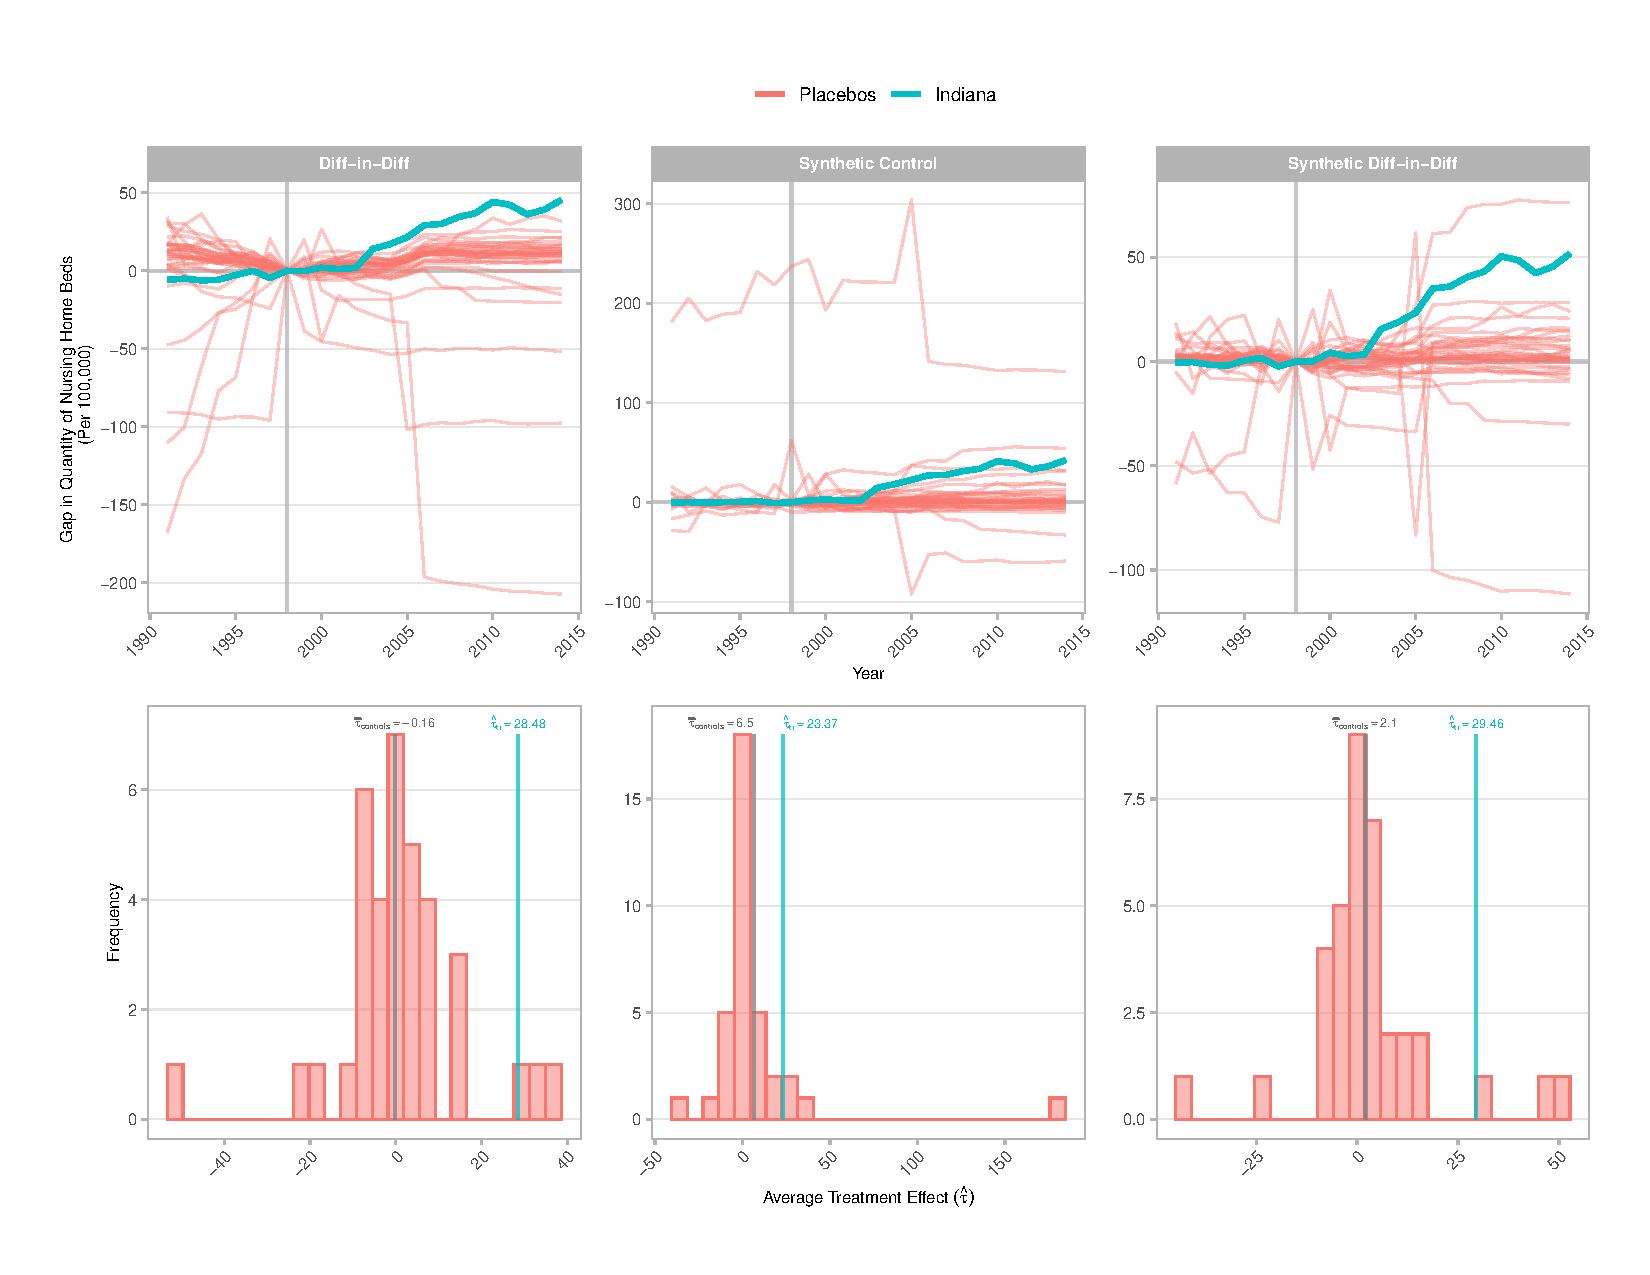
\includegraphics[width=\textwidth,keepaspectratio]{Synth_DID_Analysis/q_nhb_spag_dist_plots_IN.pdf}
    \end{center}
    \footnotesize
		\textit{Notes}: The plots in the first row show the year-specific difference in the quantity of nursing home beds per 100,000 between the ``treated'' state and its corresponding weighted average of control states. The thick blue line shows these gaps for IN, and the thin pink lines show these gaps for each of the placebo control states used in the placebo variance estimation procedure outlined in Algorithm \ref{alg:two}. To facilitate a better visual assessment of parallel trends, as well as a more meaningful comparison in how these gaps evolve over time, we make the gaps in the Diff-in-Diff and Synthetic Diff-in-Diff plots relative to their value in the year prior to IN dropping NH-CON regulations (as indicated by the vertical lines). We do not do this for the Synthetic Control plot because the SC weights are chosen to match the treated state's actual levels (as opposed to making the trends just parallel). Not normalizing the gaps for the Synthetic Control plot allows for a better assessment of the pre-treatment match between the treated state (or placebo ``treated'' state) and its respective synthetic control. The plots in the second row show the distribution of placebo estimates ($\hat{\tau}^{(b)}$ from Algorithm \ref{alg:two}), with the mean of the placebo estimates and the actual estimated effect for IN indicated by the gray and blue vertical lines, respectively. Data source: 1991-2014 Centers for Medicare and Medicaid Services’ (CMS) Provider of Services files.
\end{figure}
\clearpage

% q_nhb_plots_nd
\newpage
\begin{figure}[t] 
	\begin{center}
	\caption{\label{fig:q_nhb_plots_nd} \centering A Comparison Between DID, SC, and SDID Estimates for the Effect of Dropping NH-CON Regulations on the Quantity of Nursing Home Beds Per 100,000 in North Dakota}
    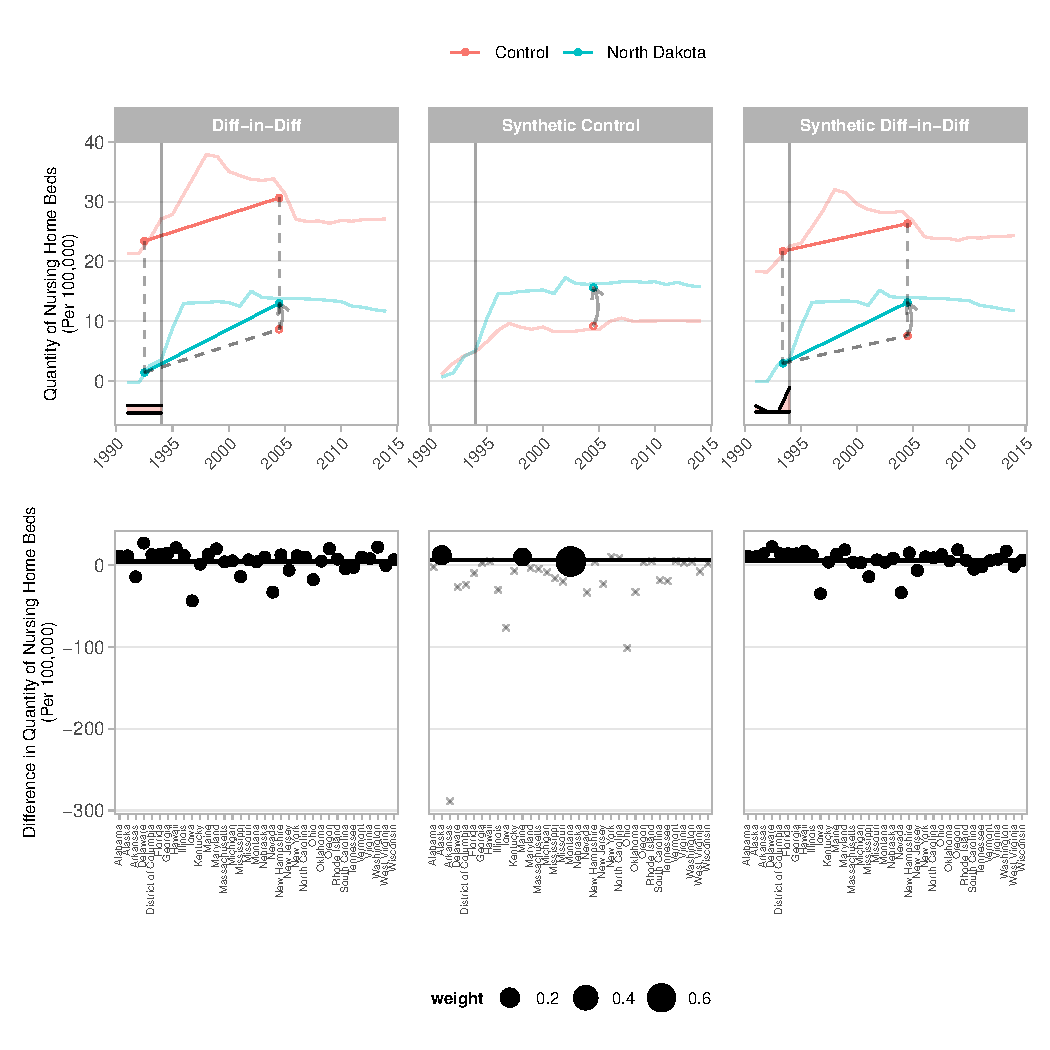
\includegraphics[width=\textwidth,keepaspectratio]{Synth_DID_Analysis/q_nursing_home_beds_plots_ND.pdf}
    \end{center}
    \footnotesize
		\textit{Notes}: The plots in the first row show trends in the quantity of nursing home beds per 100,000 over time for North Dakota and the relevant weighted average of control states, with the weights used to average pre-treatment time periods at the bottom of the plots. The curved arrows in the first row indicate the estimated average treatment effect, $\hat{\tau}$ from equation (\ref{eq:ave_effect_deltas}), and the vertical lines represent the year prior to ND dropping NH-CON regulations. The plots in the second row show the state-by-state adjusted outcome difference $\hat{\delta}_{tr}-\hat{\delta}_i$ as specified in equations (\ref{eq:sc_deltas}), (\ref{eq:did_deltas}), and (\ref{eq:sdid_deltas}), with weights $\hat{\omega}_i$ indicated by dot size, and the weighted average of these differences - the estimated effect $\hat{\tau}$ from equation (\ref{eq:ave_effect_deltas}) - indicated by the horizontal lines. Control states that get zero weight, if any, are denoted by an $\times$ symbol. Data source: 1991-2014 Centers for Medicare and Medicaid Services’ (CMS) Provider of Services files.
\end{figure}
\clearpage

% q_nhb_spag_plots_nd
\newpage
\begin{figure}[t]
	\begin{center}
	\caption{\label{fig: q_nhb_spag_plots_nd} \centering Placebo Analysis for the Effect of Dropping NH-CON Regulations on the Quantity of Nursing Home Beds Per 100,000 in North Dakota}
    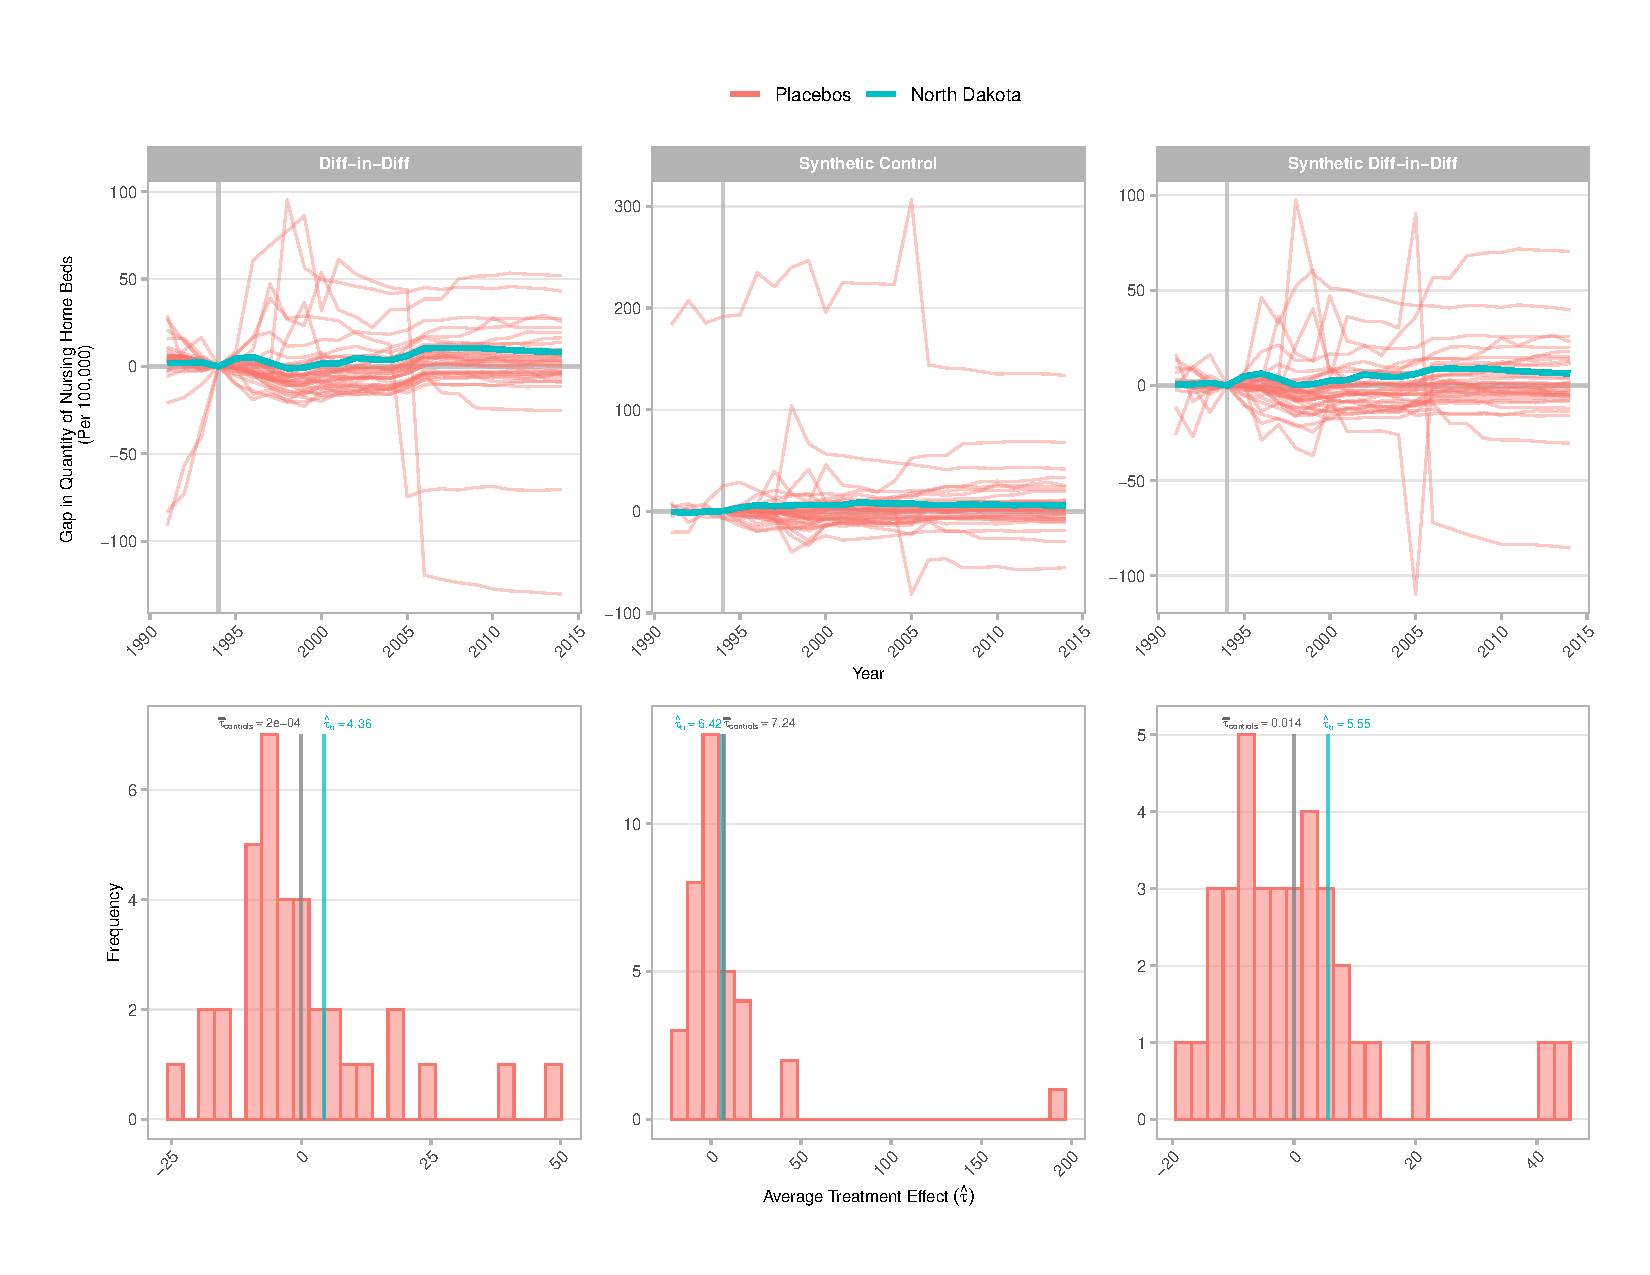
\includegraphics[width=\textwidth,keepaspectratio]{Synth_DID_Analysis/q_nhb_spag_dist_plots_ND.pdf}
    \end{center}
    \footnotesize
		\textit{Notes}: The plots in the first row show the year-specific difference in the quantity of nursing home beds per 100,000 between the ``treated'' state and its corresponding weighted average of control states. The thick blue line shows these gaps for ND, and the thin pink lines show these gaps for each of the placebo control states used in the placebo variance estimation procedure outlined in Algorithm \ref{alg:two}. To facilitate a better visual assessment of parallel trends, as well as a more meaningful comparison in how these gaps evolve over time, we make the gaps in the Diff-in-Diff and Synthetic Diff-in-Diff plots relative to their value in the year prior to ND dropping NH-CON regulations (as indicated by the vertical lines). We do not do this for the Synthetic Control plot because the SC weights are chosen to match the treated state's actual levels (as opposed to making the trends just parallel). Not normalizing the gaps for the Synthetic Control plot allows for a better assessment of the pre-treatment match between the treated state (or placebo ``treated'' state) and its respective synthetic control. The plots in the second row show the distribution of placebo estimates ($\hat{\tau}^{(b)}$ from Algorithm \ref{alg:two}), with the mean of the placebo estimates and the actual estimated effect for ND indicated by the gray and blue vertical lines, respectively. Data source: 1991-2014 Centers for Medicare and Medicaid Services’ (CMS) Provider of Services files.
\end{figure}
\clearpage



%%%%%%%%%%%%%%%%%%% Total Expenditure %%%%%%%%%%%%%%%%%%%

% tot_exp_plots_pa
\newpage
\begin{figure}[t] 
	\begin{center}
	\caption{\label{fig:tot_exp_plots_pa} \centering A Comparison Between DID, SC, and SDID Estimates for the Effect of Dropping NH-CON Regulations on Total Per Capita Nursing Home Expenditure in Pennsylvania}
    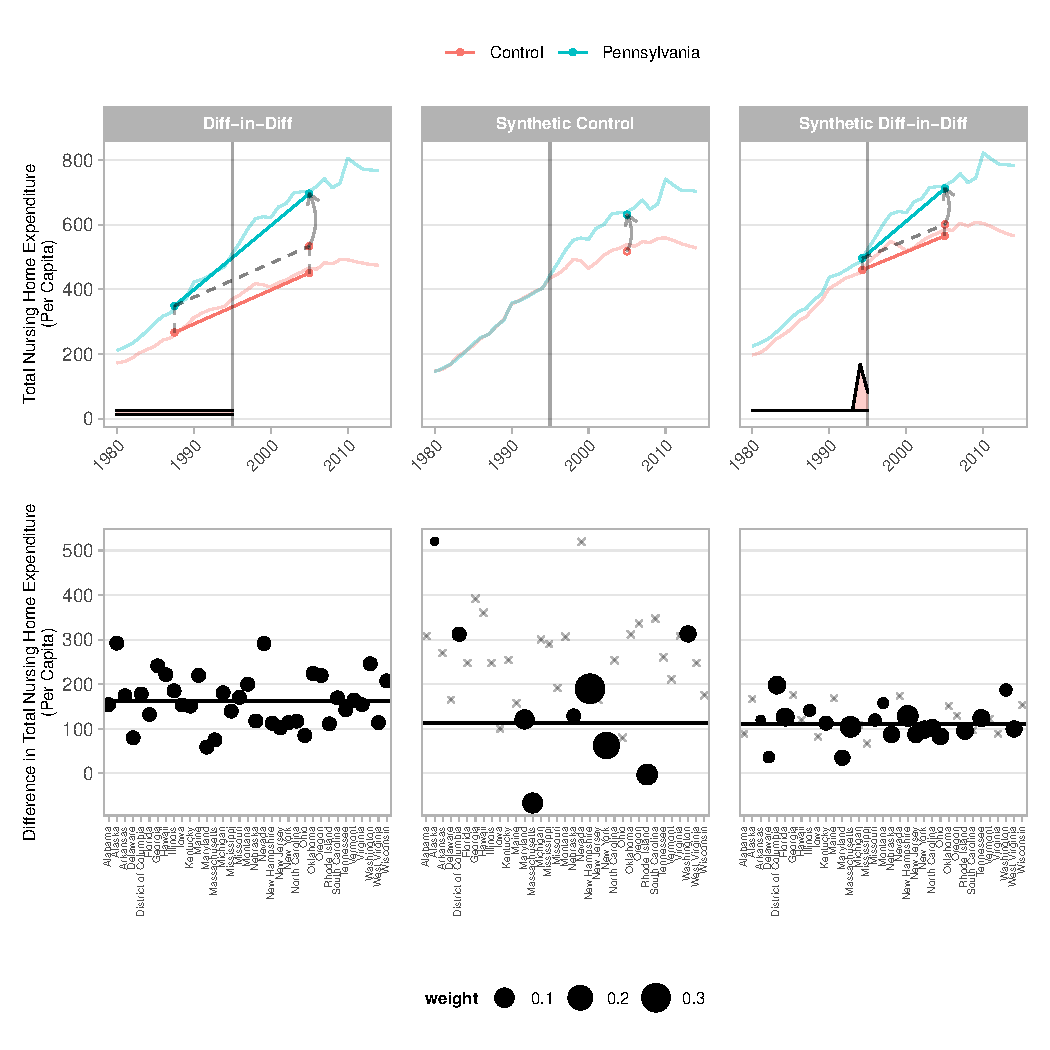
\includegraphics[width=\textwidth,keepaspectratio]{Synth_DID_Analysis/total_expenditure_plots_PA.pdf}
    \end{center}
    \footnotesize
		\textit{Notes}: The plots in the first row show trends in total per capita nursing home expenditure over time for Pennsylvania and the relevant weighted average of control states, with the weights used to average pre-treatment time periods at the bottom of the plots. The curved arrows in the first row indicate the estimated average treatment effect, $\hat{\tau}$ from equation (\ref{eq:ave_effect_deltas}), and the vertical lines represent the year prior to PA dropping NH-CON regulations. The plots in the second row show the state-by-state adjusted outcome difference $\hat{\delta}_{tr}-\hat{\delta}_i$ as specified in equations (\ref{eq:sc_deltas}), (\ref{eq:did_deltas}), and (\ref{eq:sdid_deltas}), with weights $\hat{\omega}_i$ indicated by dot size, and the weighted average of these differences - the estimated effect $\hat{\tau}$ from equation (\ref{eq:ave_effect_deltas}) - indicated by the horizontal lines. Control states that get zero weight, if any, are denoted by an $\times$ symbol. Data source: 1980-2014 National Health Expenditure Accounts (NHEA).
\end{figure}
\clearpage

% tot_exp_spag_plots_pa
\newpage
\begin{figure}[t]
	\begin{center}
	\caption{\label{fig: tot_exp_spag_plots_pa} \centering Placebo Analysis for the Effect of Dropping NH-CON Regulations on Total Per Capita Nursing Home Expenditure in Pennsylvania}
    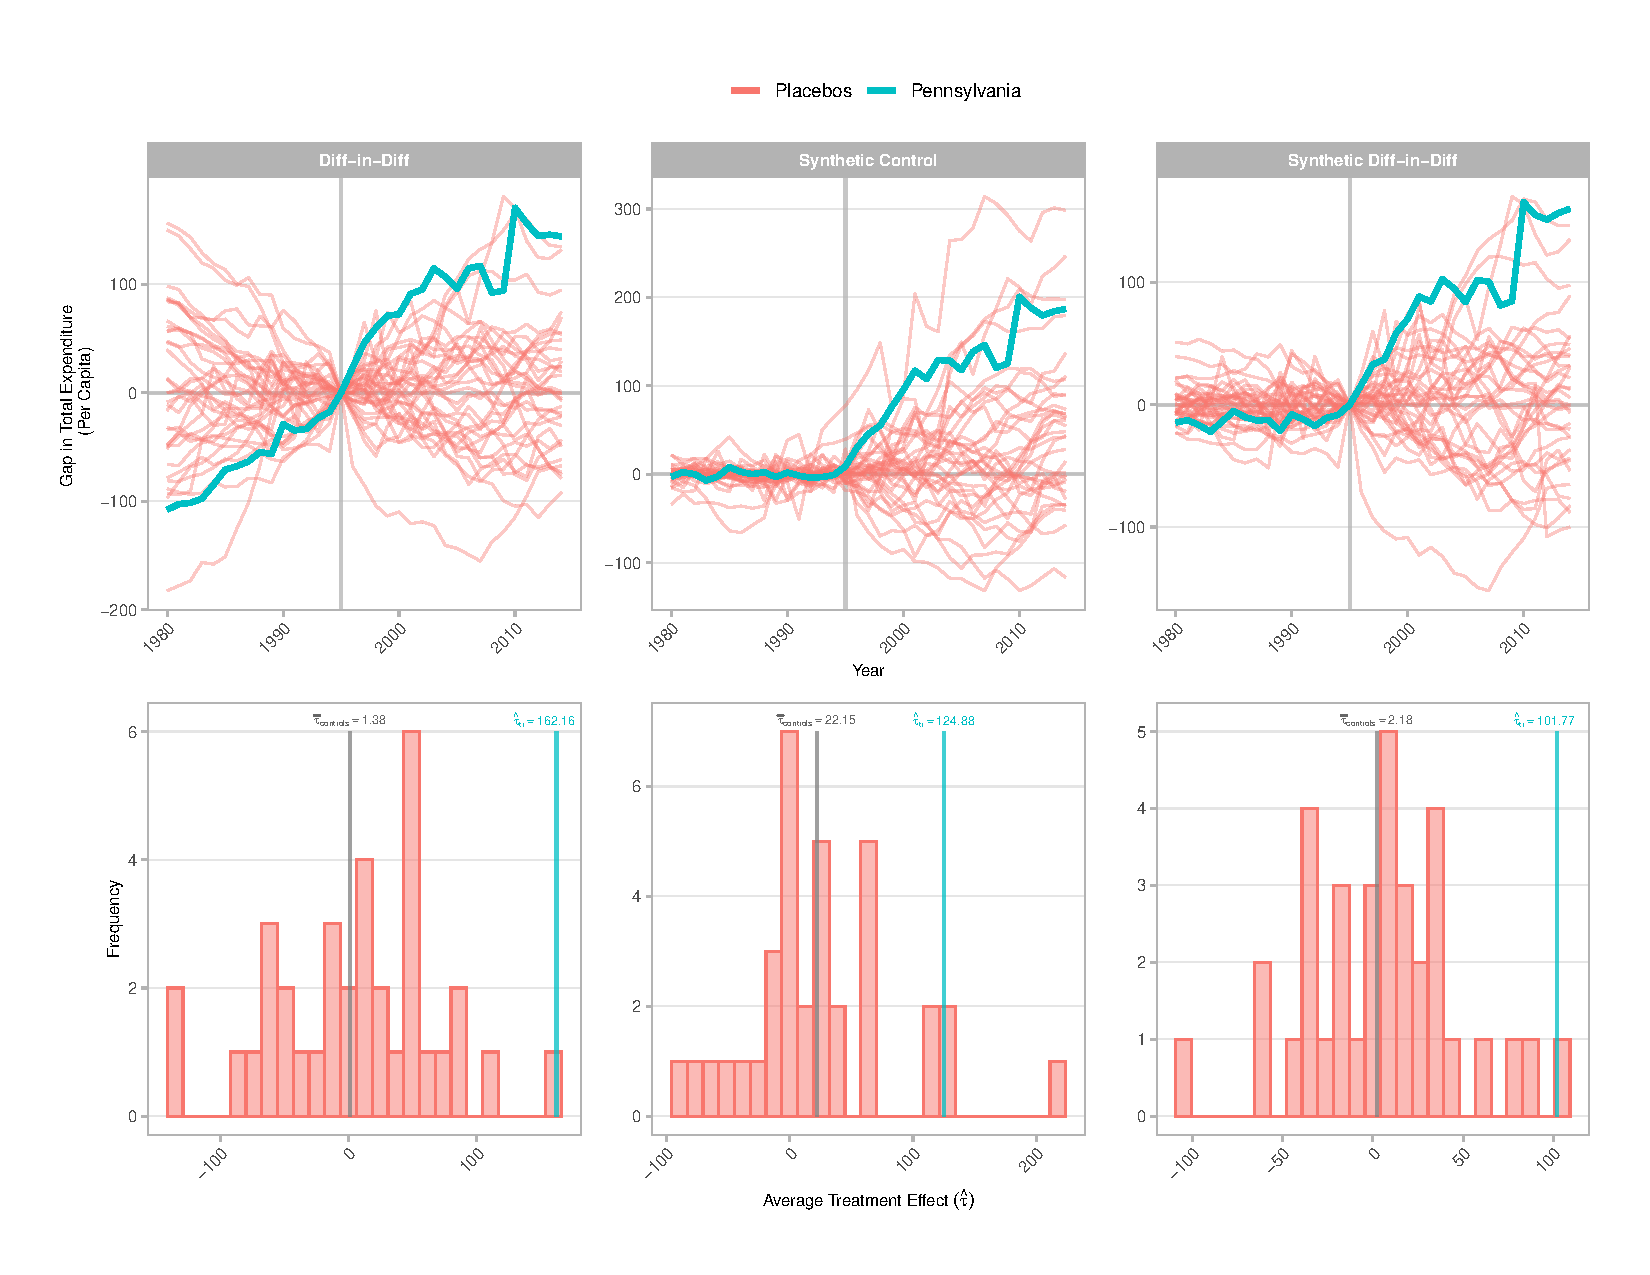
\includegraphics[width=\textwidth,keepaspectratio]{Synth_DID_Analysis/tot_exp_spag_dist_plots_PA.pdf}
    \end{center}
    \footnotesize
		\textit{Notes}: The plots in the first row show the year-specific difference in total per capita nursing home expenditure between the ``treated'' state and its corresponding weighted average of control states. The thick blue line shows these gaps for PA, and the thin pink lines show these gaps for each of the placebo control states used in the placebo variance estimation procedure outlined in Algorithm \ref{alg:two}. To facilitate a better visual assessment of parallel trends, as well as a more meaningful comparison in how these gaps evolve over time, we make the gaps in the Diff-in-Diff and Synthetic Diff-in-Diff plots relative to their value in the year prior to PA dropping NH-CON regulations (as indicated by the vertical lines). We do not do this for the Synthetic Control plot because the SC weights are chosen to match the treated state's actual levels (as opposed to making the trends just parallel). Not normalizing the gaps for the Synthetic Control plot allows for a better assessment of the pre-treatment match between the treated state (or placebo ``treated'' state) and its respective synthetic control. The plots in the second row show the distribution of placebo estimates ($\hat{\tau}^{(b)}$ from Algorithm \ref{alg:two}), with the mean of the placebo estimates and the actual estimated effect for PA indicated by the gray and blue vertical lines, respectively. Data source: 1980-2014 National Health Expenditure Accounts (NHEA).
\end{figure}
\clearpage

% tot_exp_plots_in
\newpage
\begin{figure}[t] 
	\begin{center}
	\caption{\label{fig:tot_exp_plots_in} \centering A Comparison Between DID, SC, and SDID Estimates for the Effect of Dropping NH-CON Regulations on Total Per Capita Nursing Home Expenditure in Indiana}
    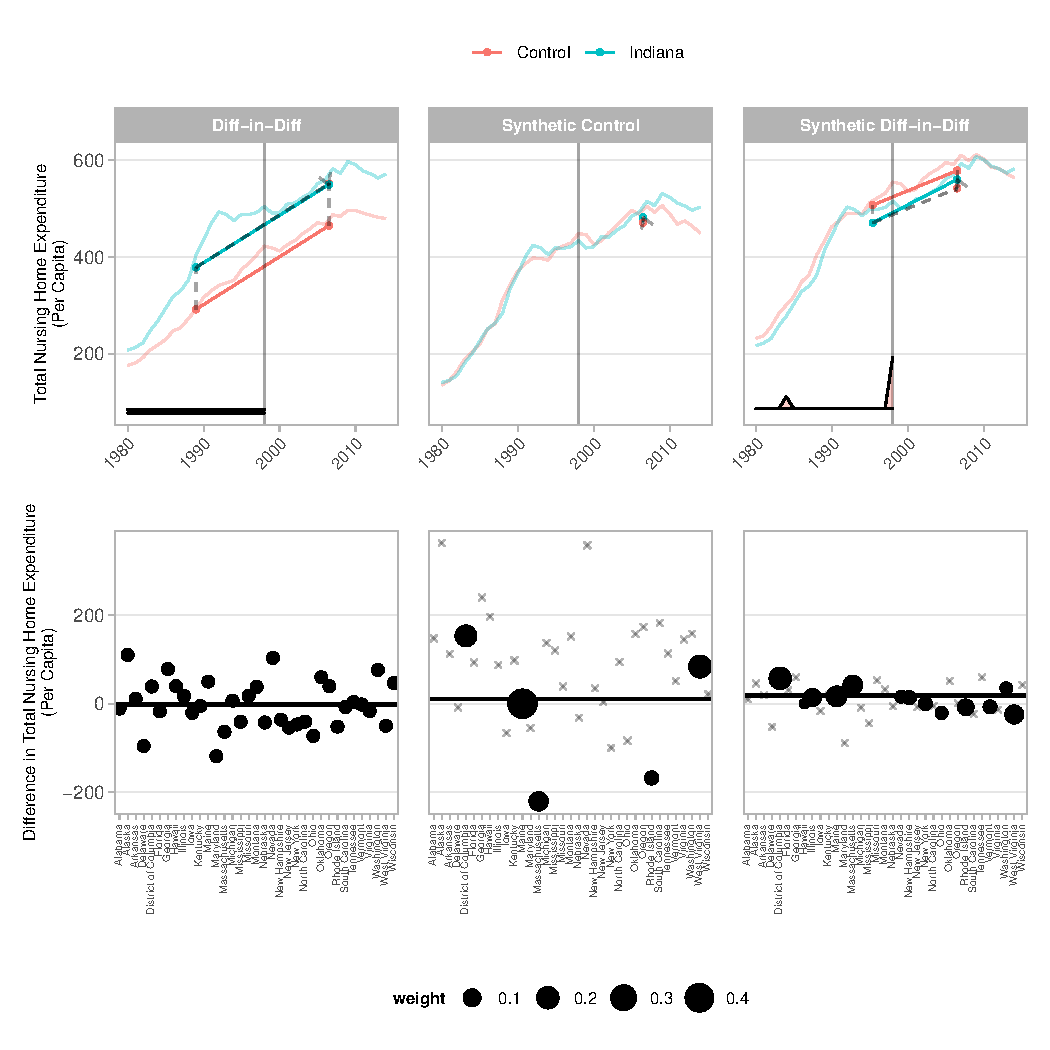
\includegraphics[width=\textwidth,keepaspectratio]{Synth_DID_Analysis/total_expenditure_plots_IN.pdf}
    \end{center}
    \footnotesize
		\textit{Notes}: The plots in the first row show trends in total per capita nursing home expenditure over time for Indiana and the relevant weighted average of control states, with the weights used to average pre-treatment time periods at the bottom of the plots. The curved arrows in the first row indicate the estimated average treatment effect, $\hat{\tau}$ from equation (\ref{eq:ave_effect_deltas}), and the vertical lines represent the year prior to IN dropping NH-CON regulations. The plots in the second row show the state-by-state adjusted outcome difference $\hat{\delta}_{tr}-\hat{\delta}_i$ as specified in equations (\ref{eq:sc_deltas}), (\ref{eq:did_deltas}), and (\ref{eq:sdid_deltas}), with weights $\hat{\omega}_i$ indicated by dot size, and the weighted average of these differences - the estimated effect $\hat{\tau}$ from equation (\ref{eq:ave_effect_deltas}) - indicated by the horizontal lines. Control states that get zero weight, if any, are denoted by an $\times$ symbol. Data source: 1980-2014 National Health Expenditure Accounts (NHEA).
\end{figure}
\clearpage

% tot_exp_spag_plots_in
\newpage
\begin{figure}[t]
	\begin{center}
	\caption{\label{fig: tot_exp_spag_plots_in} \centering Placebo Analysis for the Effect of Dropping NH-CON Regulations on Total Per Capita Nursing Home Expenditure in Indiana}
    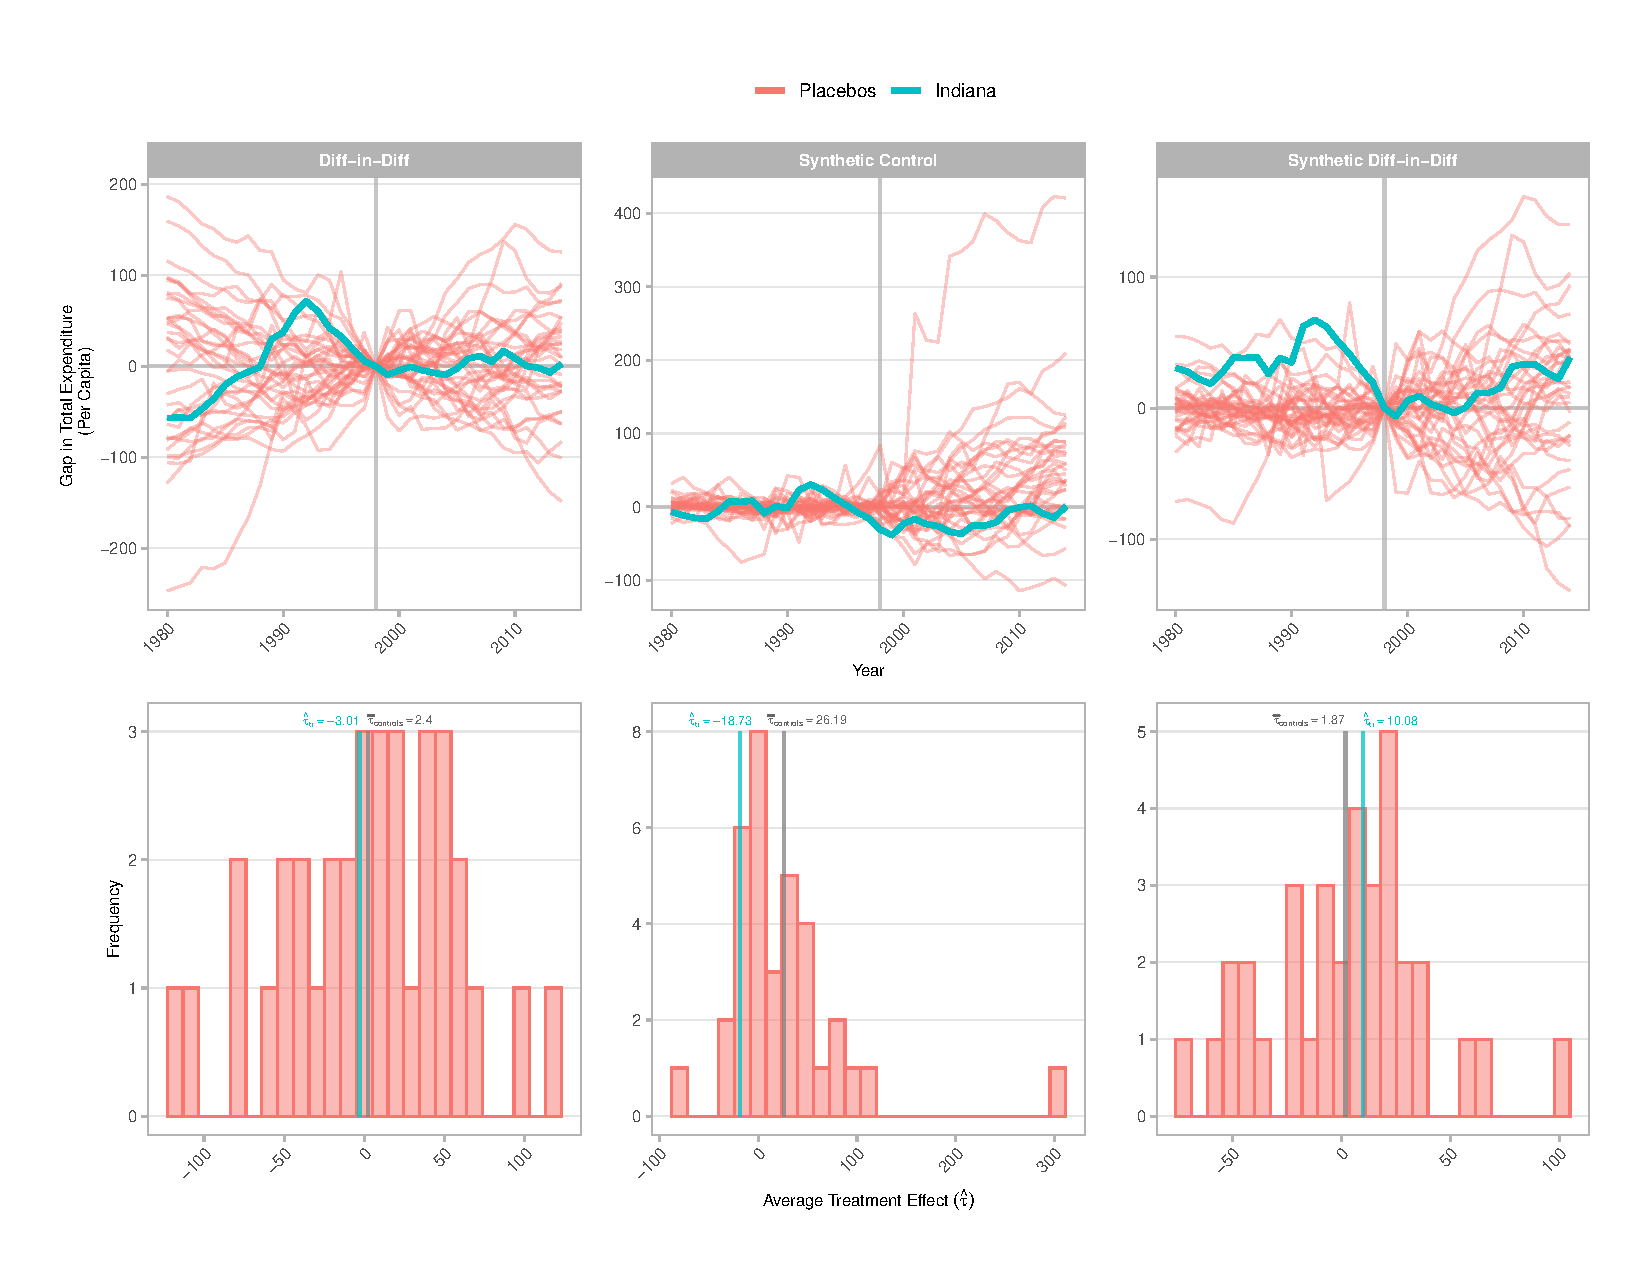
\includegraphics[width=\textwidth,keepaspectratio]{Synth_DID_Analysis/tot_exp_spag_dist_plots_IN.pdf}
    \end{center}
    \footnotesize
		\textit{Notes}: The plots in the first row show the year-specific difference in total per capita nursing home expenditure between the ``treated'' state and its corresponding weighted average of control states. The thick blue line shows these gaps for IN, and the thin pink lines show these gaps for each of the placebo control states used in the placebo variance estimation procedure outlined in Algorithm \ref{alg:two}. To facilitate a better visual assessment of parallel trends, as well as a more meaningful comparison in how these gaps evolve over time, we make the gaps in the Diff-in-Diff and Synthetic Diff-in-Diff plots relative to their value in the year prior to IN dropping NH-CON regulations (as indicated by the vertical lines). We do not do this for the Synthetic Control plot because the SC weights are chosen to match the treated state's actual levels (as opposed to making the trends just parallel). Not normalizing the gaps for the Synthetic Control plot allows for a better assessment of the pre-treatment match between the treated state (or placebo ``treated'' state) and its respective synthetic control. The plots in the second row show the distribution of placebo estimates ($\hat{\tau}^{(b)}$ from Algorithm \ref{alg:two}), with the mean of the placebo estimates and the actual estimated effect for IN indicated by the gray and blue vertical lines, respectively. Data source: 1980-2014 National Health Expenditure Accounts (NHEA).
\end{figure}
\clearpage

% tot_exp_plots_nd
\newpage
\begin{figure}[t] 
	\begin{center}
	\caption{\label{fig:tot_exp_plots_nd} \centering A Comparison Between DID, SC, and SDID Estimates for the Effect of Dropping NH-CON Regulations on Total Per Capita Nursing Home Expenditure in North Dakota}
    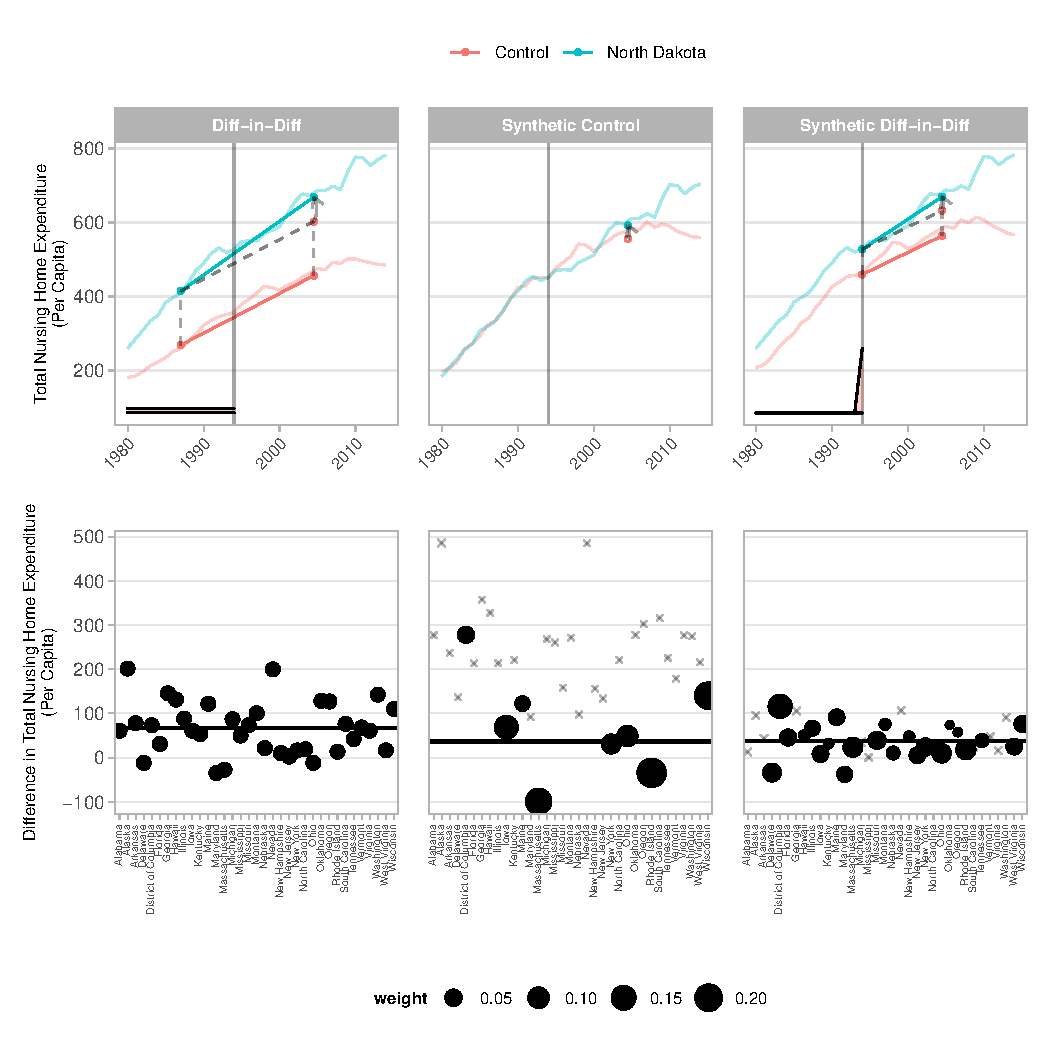
\includegraphics[width=\textwidth,keepaspectratio]{Synth_DID_Analysis/total_expenditure_plots_ND.pdf}
    \end{center}
    \footnotesize
		\textit{Notes}: The plots in the first row show trends in total per capita nursing home expenditure over time for North Dakota and the relevant weighted average of control states, with the weights used to average pre-treatment time periods at the bottom of the plots. The curved arrows in the first row indicate the estimated average treatment effect, $\hat{\tau}$ from equation (\ref{eq:ave_effect_deltas}), and the vertical lines represent the year prior to ND dropping NH-CON regulations. The plots in the second row show the state-by-state adjusted outcome difference $\hat{\delta}_{tr}-\hat{\delta}_i$ as specified in equations (\ref{eq:sc_deltas}), (\ref{eq:did_deltas}), and (\ref{eq:sdid_deltas}), with weights $\hat{\omega}_i$ indicated by dot size, and the weighted average of these differences - the estimated effect $\hat{\tau}$ from equation (\ref{eq:ave_effect_deltas}) - indicated by the horizontal lines. Control states that get zero weight, if any, are denoted by an $\times$ symbol. Data source: 1980-2014 National Health Expenditure Accounts (NHEA).
\end{figure}
\clearpage

% tot_exp_spag_plots_nd
\newpage
\begin{figure}[t]
	\begin{center}
	\caption{\label{fig: tot_exp_spag_plots_nd} \centering Placebo Analysis for the Effect of Dropping NH-CON Regulations on Total Per Capita Nursing Home Expenditure in North Dakota}
    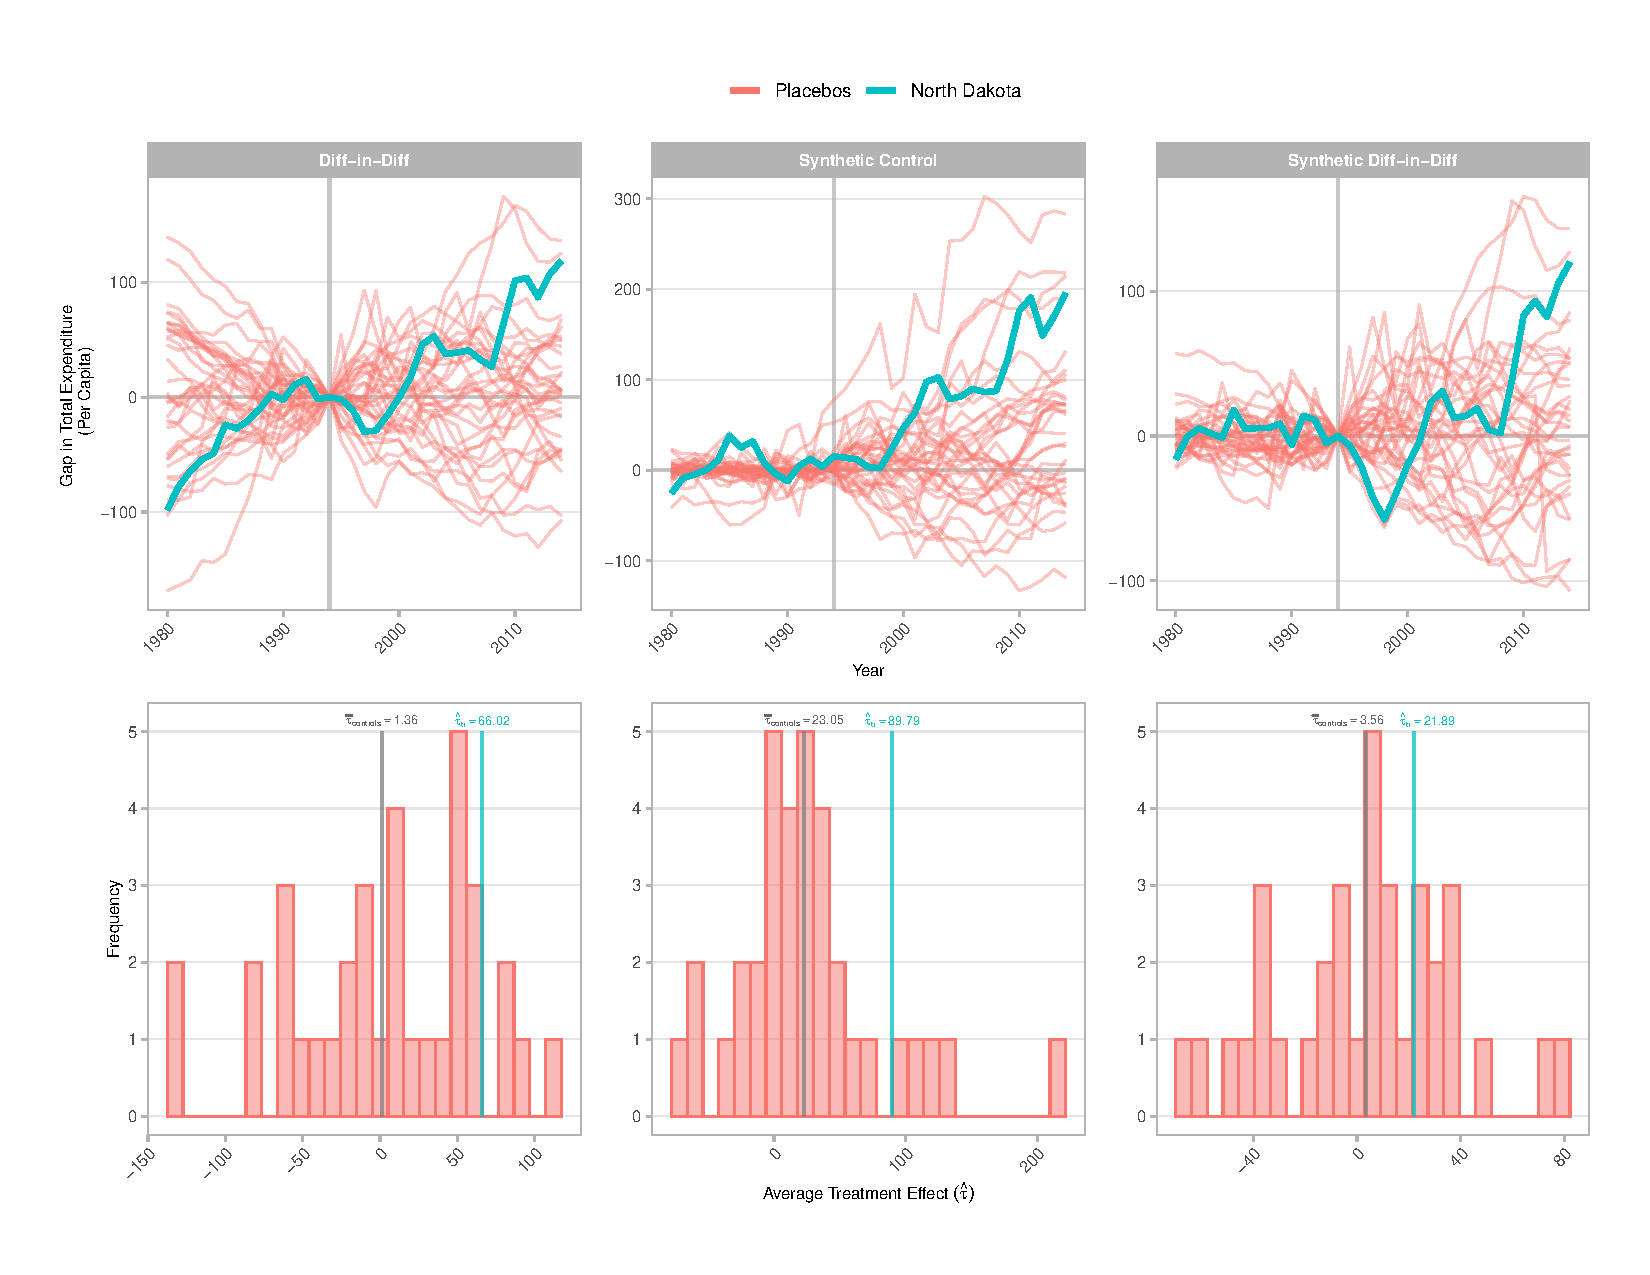
\includegraphics[width=\textwidth,keepaspectratio]{Synth_DID_Analysis/tot_exp_spag_dist_plots_ND.pdf}
    \end{center}
    \footnotesize
		\textit{Notes}: The plots in the first row show the year-specific difference in total per capita nursing home expenditure between the ``treated'' state and its corresponding weighted average of control states. The thick blue line shows these gaps for ND, and the thin pink lines show these gaps for each of the placebo control states used in the placebo variance estimation procedure outlined in Algorithm \ref{alg:two}. To facilitate a better visual assessment of parallel trends, as well as a more meaningful comparison in how these gaps evolve over time, we make the gaps in the Diff-in-Diff and Synthetic Diff-in-Diff plots relative to their value in the year prior to ND dropping NH-CON regulations (as indicated by the vertical lines). We do not do this for the Synthetic Control plot because the SC weights are chosen to match the treated state's actual levels (as opposed to making the trends just parallel). Not normalizing the gaps for the Synthetic Control plot allows for a better assessment of the pre-treatment match between the treated state (or placebo ``treated'' state) and its respective synthetic control. The plots in the second row show the distribution of placebo estimates ($\hat{\tau}^{(b)}$ from Algorithm \ref{alg:two}), with the mean of the placebo estimates and the actual estimated effect for ND indicated by the gray and blue vertical lines, respectively. Data source: 1980-2014 National Health Expenditure Accounts (NHEA).
\end{figure}
\clearpage




%%%%%%%%%%%%%%%%%%% Medicaid Expenditure %%%%%%%%%%%%%%%%%%%

% med_exp_plots_pa
\newpage
\begin{figure}[t] 
	\begin{center}
	\caption{\label{fig:med_exp_plots_pa} \centering A Comparison Between DID, SC, and SDID Estimates for the Effect of Dropping NH-CON Regulations on Per Capita Medicaid Nursing Home Expenditure in Pennsylvania}
    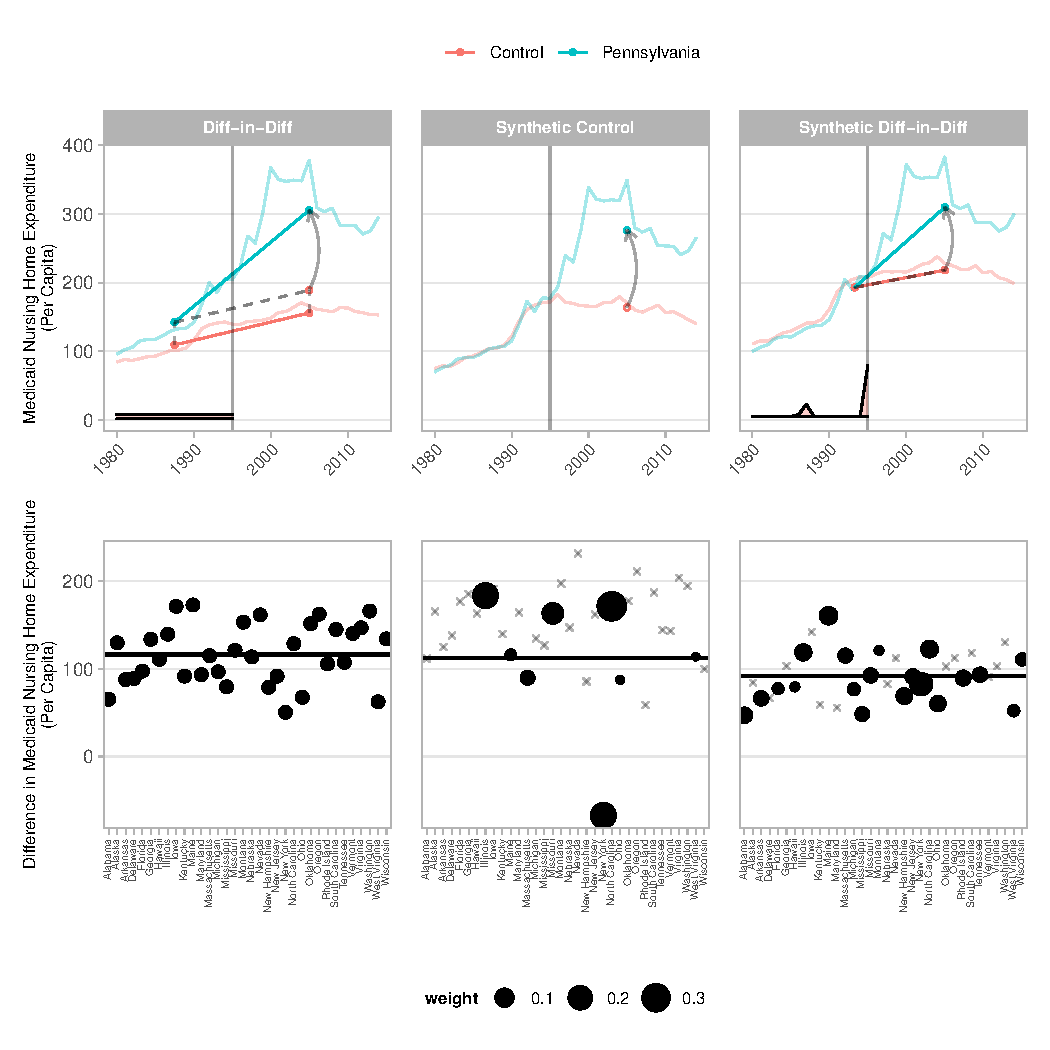
\includegraphics[width=\textwidth,keepaspectratio]{Synth_DID_Analysis/medicaid_expenditure_plots_PA.pdf}
    \end{center}
    \footnotesize
		\textit{Notes}: The plots in the first row show trends in per capita Medicaid nursing home expenditure over time for Pennsylvania and the relevant weighted average of control states, with the weights used to average pre-treatment time periods at the bottom of the plots. The curved arrows in the first row indicate the estimated average treatment effect, $\hat{\tau}$ from equation (\ref{eq:ave_effect_deltas}), and the vertical lines represent the year prior to PA dropping NH-CON regulations. The plots in the second row show the state-by-state adjusted outcome difference $\hat{\delta}_{tr}-\hat{\delta}_i$ as specified in equations (\ref{eq:sc_deltas}), (\ref{eq:did_deltas}), and (\ref{eq:sdid_deltas}), with weights $\hat{\omega}_i$ indicated by dot size, and the weighted average of these differences - the estimated effect $\hat{\tau}$ from equation (\ref{eq:ave_effect_deltas}) - indicated by the horizontal lines. Control states that get zero weight, if any, are denoted by an $\times$ symbol. Data source: 1980-2014 National Health Expenditure Accounts (NHEA).
\end{figure}
\clearpage

% med_exp_spag_plots_pa
\newpage
\begin{figure}[t]
	\begin{center}
	\caption{\label{fig: med_exp_spag_plots_pa} \centering Placebo Analysis for the Effect of Dropping NH-CON Regulations on Per Capita Medicaid Nursing Home Expenditure in Pennsylvania}
    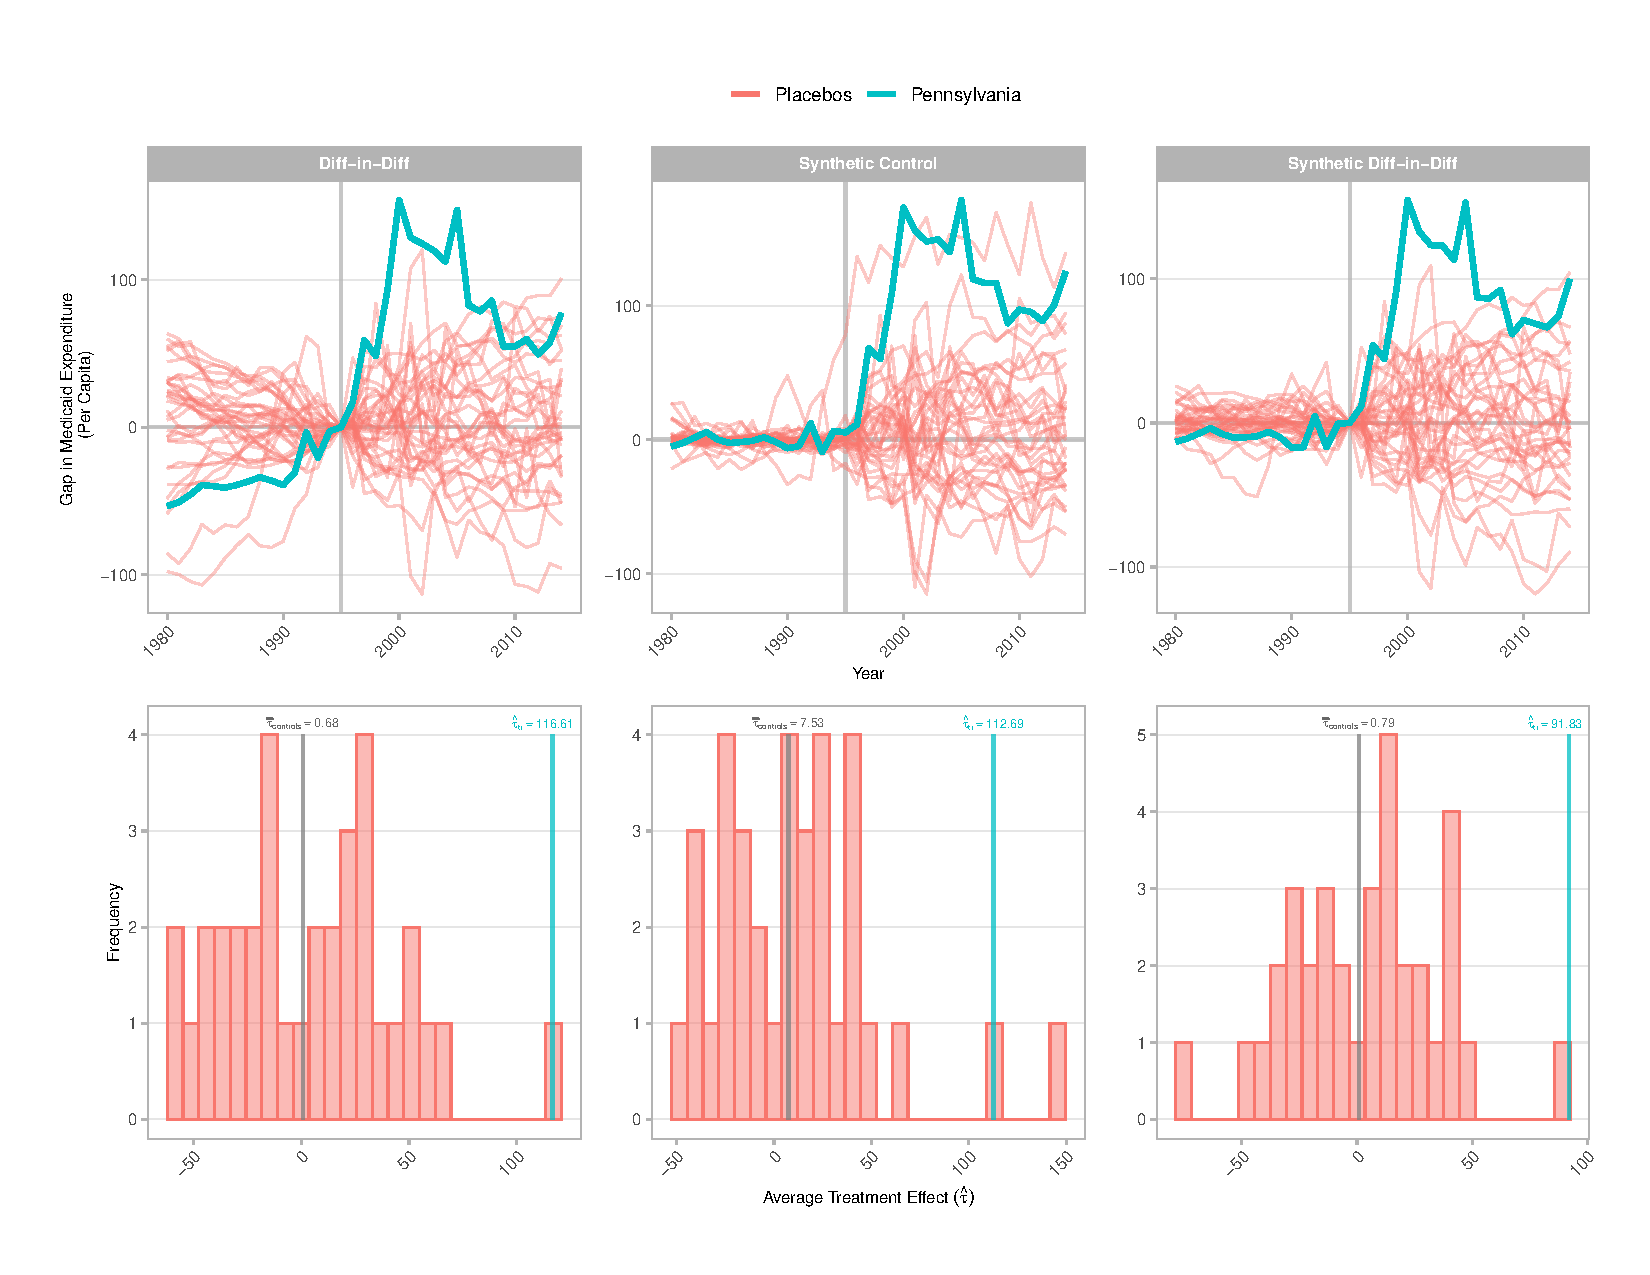
\includegraphics[width=\textwidth,keepaspectratio]{Synth_DID_Analysis/med_exp_spag_dist_plots_PA.pdf}
    \end{center}
    \footnotesize
		\textit{Notes}: The plots in the first row show the year-specific difference in per capita Medicaid nursing home expenditure between the ``treated'' state and its corresponding weighted average of control states. The thick blue line shows these gaps for PA, and the thin pink lines show these gaps for each of the placebo control states used in the placebo variance estimation procedure outlined in Algorithm \ref{alg:two}. To facilitate a better visual assessment of parallel trends, as well as a more meaningful comparison in how these gaps evolve over time, we make the gaps in the Diff-in-Diff and Synthetic Diff-in-Diff plots relative to their value in the year prior to PA dropping NH-CON regulations (as indicated by the vertical lines). We do not do this for the Synthetic Control plot because the SC weights are chosen to match the treated state's actual levels (as opposed to making the trends just parallel). Not normalizing the gaps for the Synthetic Control plot allows for a better assessment of the pre-treatment match between the treated state (or placebo ``treated'' state) and its respective synthetic control. The plots in the second row show the distribution of placebo estimates ($\hat{\tau}^{(b)}$ from Algorithm \ref{alg:two}), with the mean of the placebo estimates and the actual estimated effect for PA indicated by the gray and blue vertical lines, respectively. Data source: 1980-2014 National Health Expenditure Accounts (NHEA).
\end{figure}
\clearpage

% med_exp_plots_in
\newpage
\begin{figure}[t] 
	\begin{center}
	\caption{\label{fig:med_exp_plots_in} \centering A Comparison Between DID, SC, and SDID Estimates for the Effect of Dropping NH-CON Regulations on Per Capita Medicaid Nursing Home Expenditure in Indiana}
    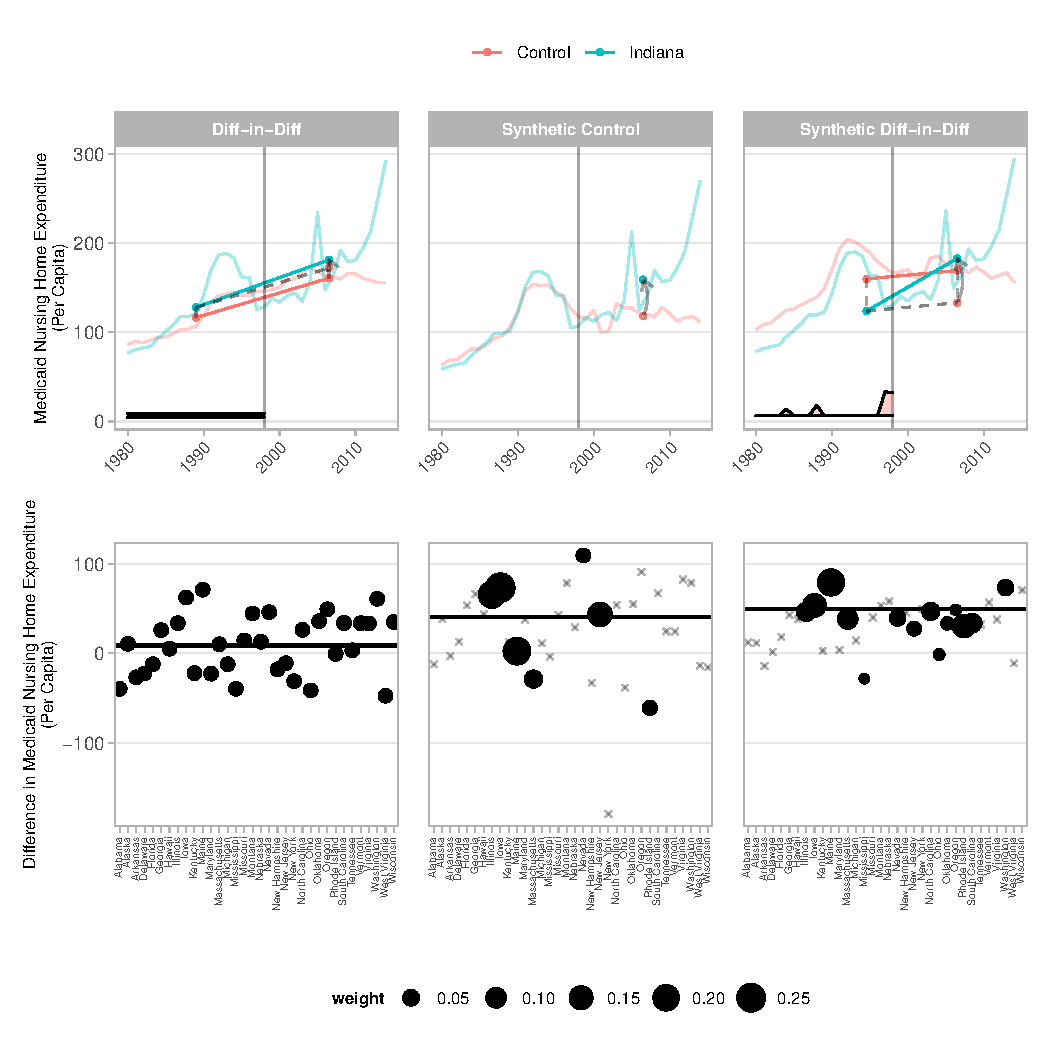
\includegraphics[width=\textwidth,keepaspectratio]{Synth_DID_Analysis/medicaid_expenditure_plots_IN.pdf}
    \end{center}
    \footnotesize
		\textit{Notes}: The plots in the first row show trends in per capita Medicaid nursing home expenditure over time for Indiana and the relevant weighted average of control states, with the weights used to average pre-treatment time periods at the bottom of the plots. The curved arrows in the first row indicate the estimated average treatment effect, $\hat{\tau}$ from equation (\ref{eq:ave_effect_deltas}), and the vertical lines represent the year prior to IN dropping NH-CON regulations. The plots in the second row show the state-by-state adjusted outcome difference $\hat{\delta}_{tr}-\hat{\delta}_i$ as specified in equations (\ref{eq:sc_deltas}), (\ref{eq:did_deltas}), and (\ref{eq:sdid_deltas}), with weights $\hat{\omega}_i$ indicated by dot size, and the weighted average of these differences - the estimated effect $\hat{\tau}$ from equation (\ref{eq:ave_effect_deltas}) - indicated by the horizontal lines. Control states that get zero weight, if any, are denoted by an $\times$ symbol. Data source: 1980-2014 National Health Expenditure Accounts (NHEA).
\end{figure}
\clearpage

% med_exp_spag_plots_in
\newpage
\begin{figure}[t]
	\begin{center}
	\caption{\label{fig: med_exp_spag_plots_in} \centering Placebo Analysis for the Effect of Dropping NH-CON Regulations on Per Capita Medicaid Nursing Home Expenditure in Indiana}
    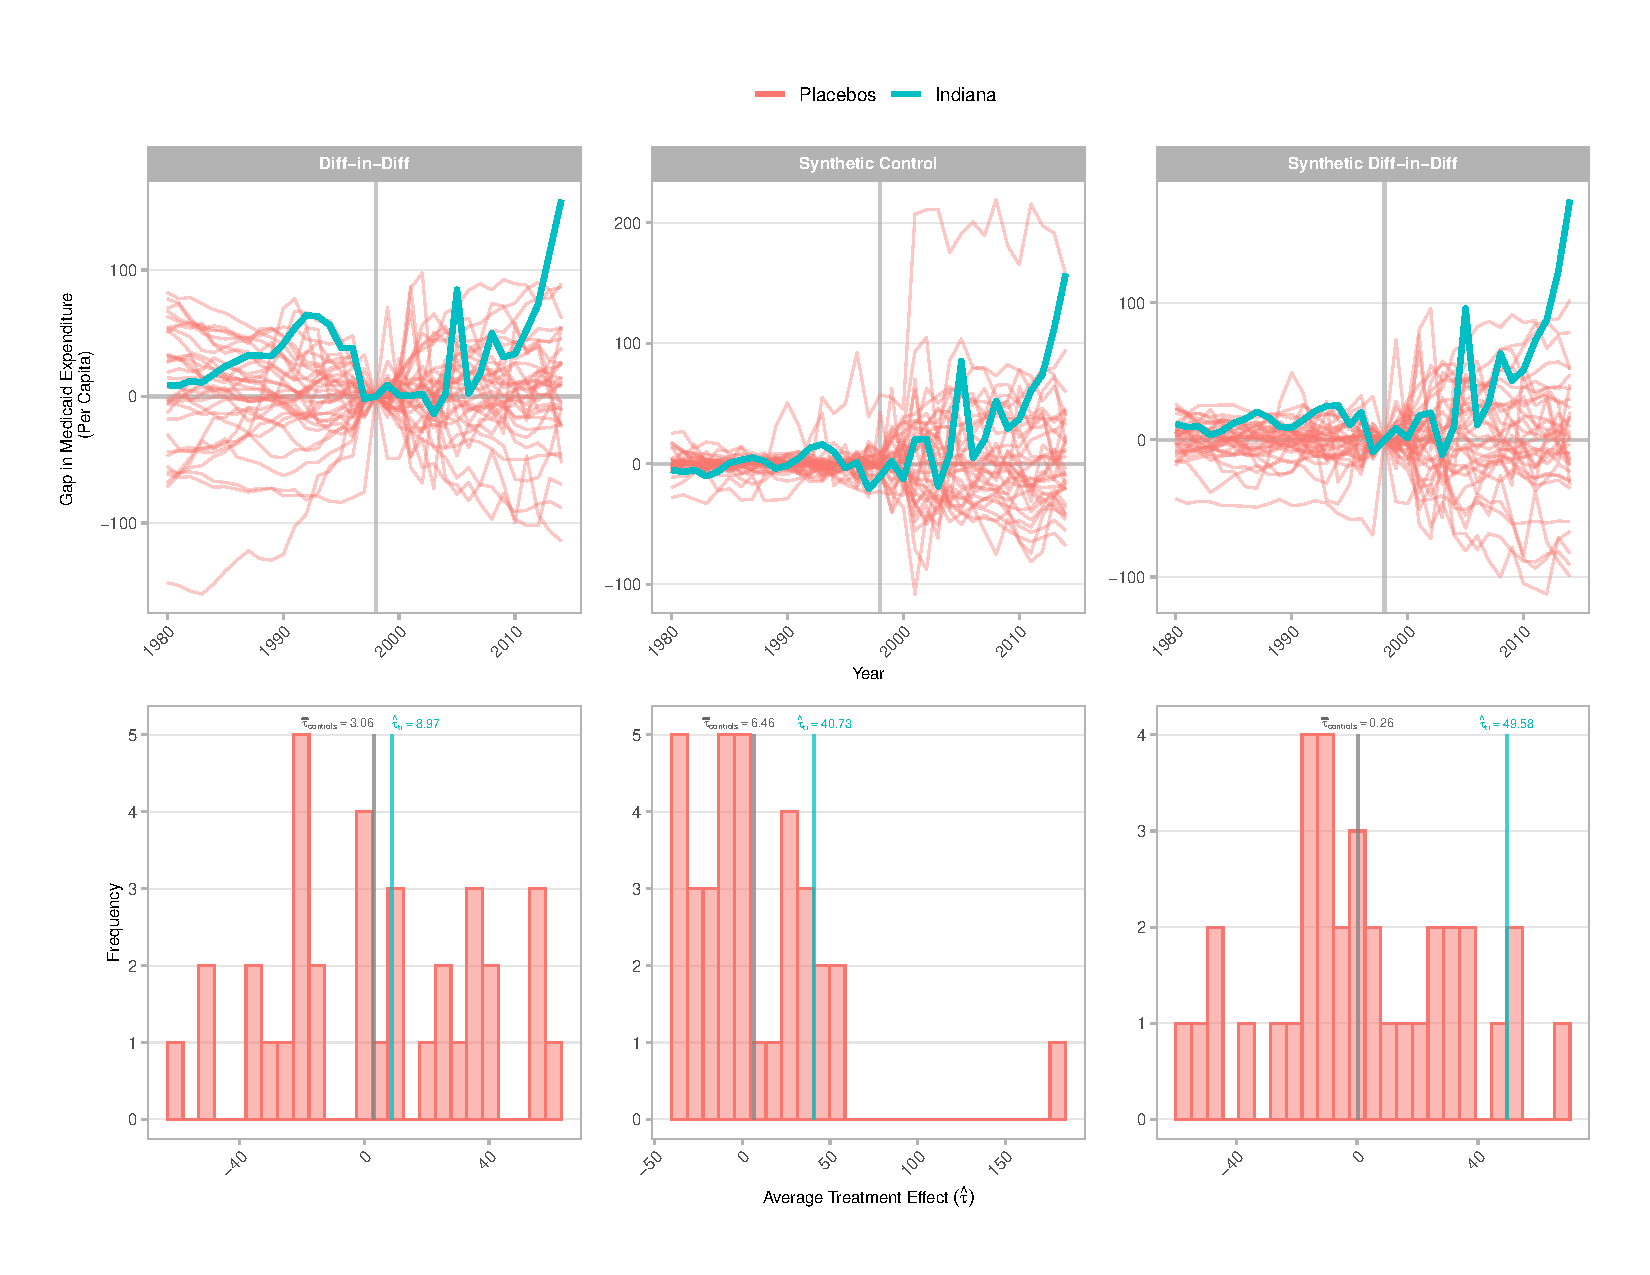
\includegraphics[width=\textwidth,keepaspectratio]{Synth_DID_Analysis/med_exp_spag_dist_plots_IN.pdf}
    \end{center}
    \footnotesize
		\textit{Notes}: The plots in the first row show the year-specific difference in per capita Medicaid nursing home expenditure between the ``treated'' state and its corresponding weighted average of control states. The thick blue line shows these gaps for IN, and the thin pink lines show these gaps for each of the placebo control states used in the placebo variance estimation procedure outlined in Algorithm \ref{alg:two}. To facilitate a better visual assessment of parallel trends, as well as a more meaningful comparison in how these gaps evolve over time, we make the gaps in the Diff-in-Diff and Synthetic Diff-in-Diff plots relative to their value in the year prior to IN dropping NH-CON regulations (as indicated by the vertical lines). We do not do this for the Synthetic Control plot because the SC weights are chosen to match the treated state's actual levels (as opposed to making the trends just parallel). Not normalizing the gaps for the Synthetic Control plot allows for a better assessment of the pre-treatment match between the treated state (or placebo ``treated'' state) and its respective synthetic control. The plots in the second row show the distribution of placebo estimates ($\hat{\tau}^{(b)}$ from Algorithm \ref{alg:two}), with the mean of the placebo estimates and the actual estimated effect for IN indicated by the gray and blue vertical lines, respectively. Data source: 1980-2014 National Health Expenditure Accounts (NHEA).
\end{figure}
\clearpage

% med_exp_plots_nd
\newpage
\begin{figure}[t] 
	\begin{center}
	\caption{\label{fig:med_exp_plots_nd} \centering A Comparison Between DID, SC, and SDID Estimates for the Effect of Dropping NH-CON Regulations on Per Capita Medicaid Nursing Home Expenditure in North Dakota}
    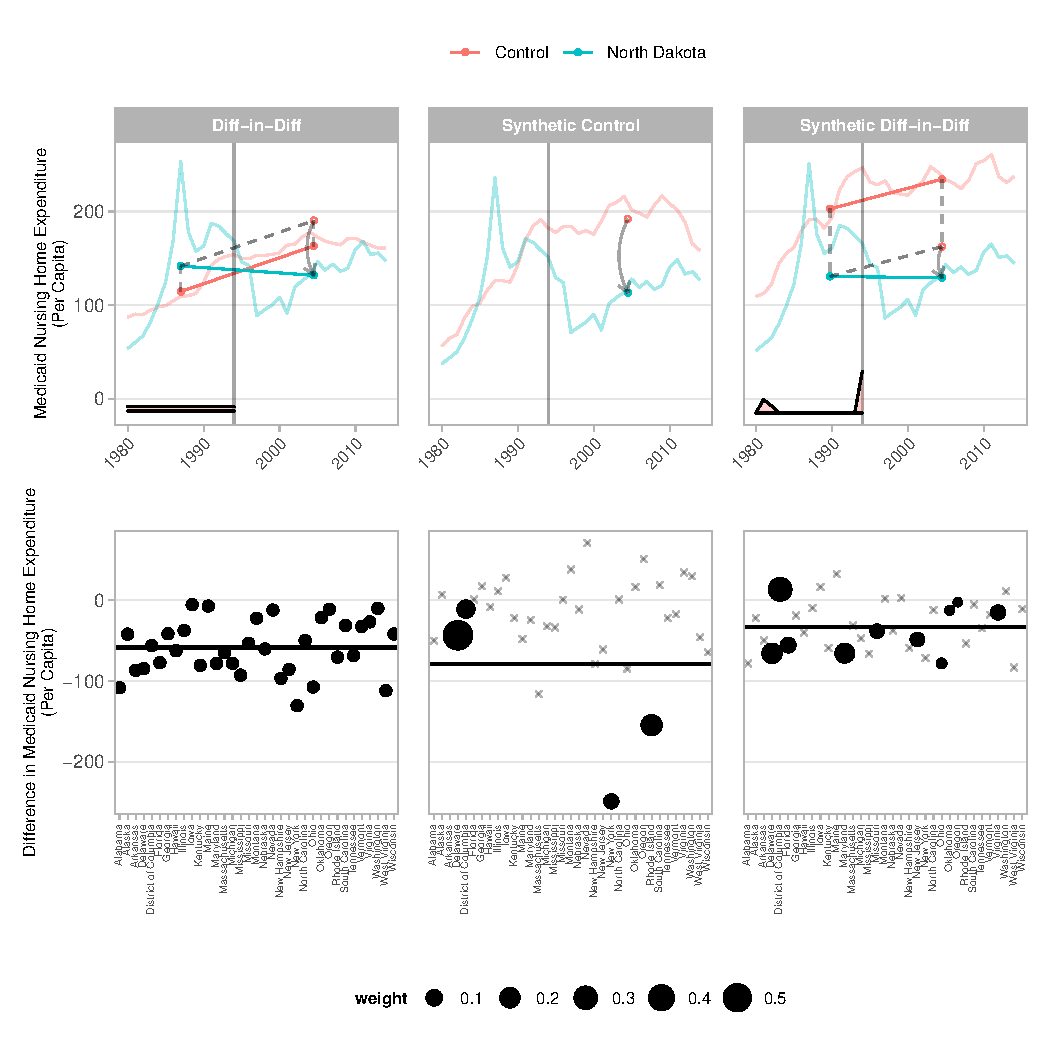
\includegraphics[width=\textwidth,keepaspectratio]{Synth_DID_Analysis/medicaid_expenditure_plots_ND.pdf}
    \end{center}
    \footnotesize
		\textit{Notes}: The plots in the first row show trends in per capita Medicaid nursing home expenditure over time for North Dakota and the relevant weighted average of control states, with the weights used to average pre-treatment time periods at the bottom of the plots. The curved arrows in the first row indicate the estimated average treatment effect, $\hat{\tau}$ from equation (\ref{eq:ave_effect_deltas}), and the vertical lines represent the year prior to ND dropping NH-CON regulations. The plots in the second row show the state-by-state adjusted outcome difference $\hat{\delta}_{tr}-\hat{\delta}_i$ as specified in equations (\ref{eq:sc_deltas}), (\ref{eq:did_deltas}), and (\ref{eq:sdid_deltas}), with weights $\hat{\omega}_i$ indicated by dot size, and the weighted average of these differences - the estimated effect $\hat{\tau}$ from equation (\ref{eq:ave_effect_deltas}) - indicated by the horizontal lines. Control states that get zero weight, if any, are denoted by an $\times$ symbol. Data source: 1980-2014 National Health Expenditure Accounts (NHEA).
\end{figure}
\clearpage

% med_exp_spag_plots_nd
\newpage
\begin{figure}[t]
	\begin{center}
	\caption{\label{fig: med_exp_spag_plots_nd} \centering Placebo Analysis for the Effect of Dropping NH-CON Regulations on Per Capita Medicaid Nursing Home Expenditure in North Dakota}
    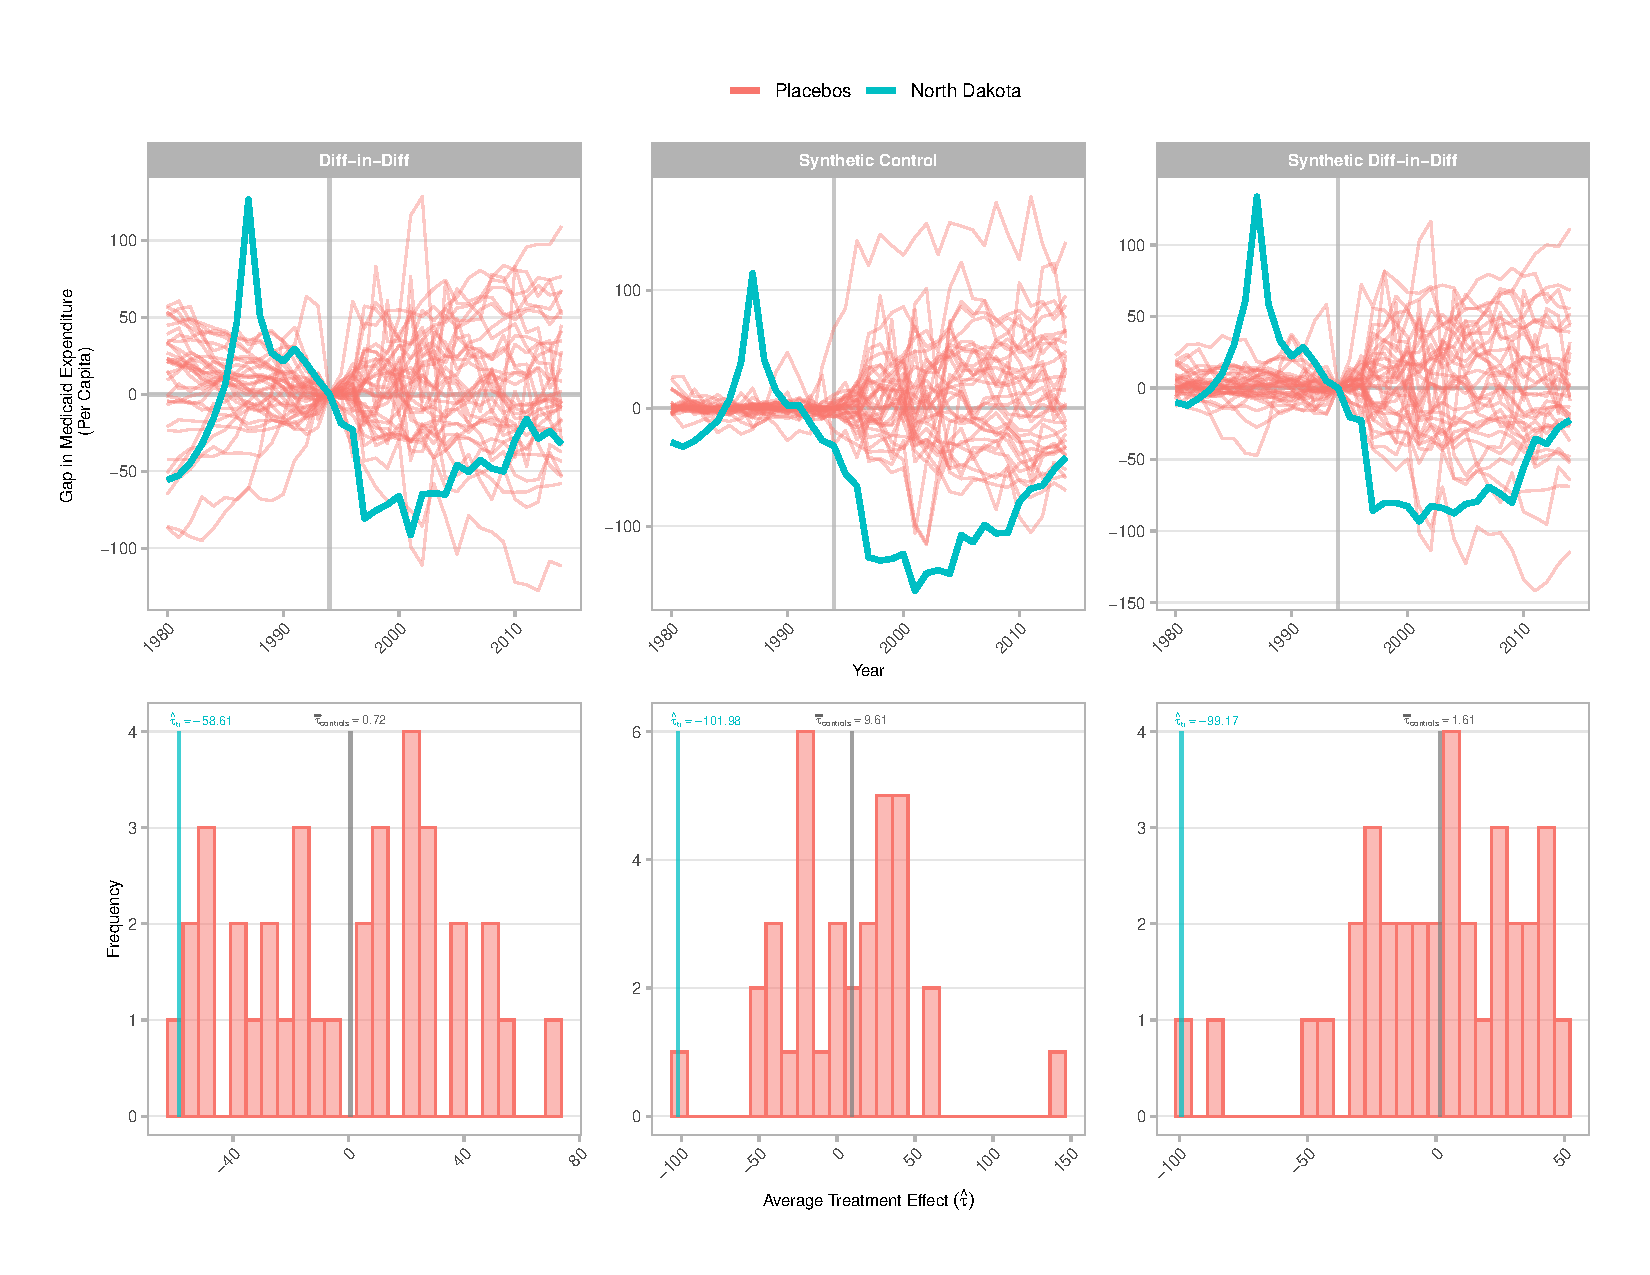
\includegraphics[width=\textwidth,keepaspectratio]{Synth_DID_Analysis/med_exp_spag_dist_plots_ND.pdf}
    \end{center}
    \footnotesize
		\textit{Notes}: The plots in the first row show the year-specific difference in per capita Medicaid nursing home expenditure between the ``treated'' state and its corresponding weighted average of control states. The thick blue line shows these gaps for ND, and the thin pink lines show these gaps for each of the placebo control states used in the placebo variance estimation procedure outlined in Algorithm \ref{alg:two}. To facilitate a better visual assessment of parallel trends, as well as a more meaningful comparison in how these gaps evolve over time, we make the gaps in the Diff-in-Diff and Synthetic Diff-in-Diff plots relative to their value in the year prior to ND dropping NH-CON regulations (as indicated by the vertical lines). We do not do this for the Synthetic Control plot because the SC weights are chosen to match the treated state's actual levels (as opposed to making the trends just parallel). Not normalizing the gaps for the Synthetic Control plot allows for a better assessment of the pre-treatment match between the treated state (or placebo ``treated'' state) and its respective synthetic control. The plots in the second row show the distribution of placebo estimates ($\hat{\tau}^{(b)}$ from Algorithm \ref{alg:two}), with the mean of the placebo estimates and the actual estimated effect for ND indicated by the gray and blue vertical lines, respectively. Data source: 1980-2014 National Health Expenditure Accounts (NHEA).
\end{figure}
\clearpage




\end{document}